
In order to verify the feasibility of the proposed load balancer architecture, we evaluated it with the following criteria;
(1) Basic functionality and Portability:
We evaluated the load balancer functionality using physical servers in on-premise data center and compared performance level with existing iptables DNAT and nginx as a load balancer.
We also carried out the same performance measurement in GCP and AWS to show the containerized ipvs load balancer is runnable even in the cloud environment.
(2) Redundancy and Scalability:
We evaluated ECMP functionality by watching routing table updates on the router when the new load balancer is added or removed.
We also evaluated the performance level by changing the number of load balancers.
%
The following subsections explain the evaluation in detail.

\section{Performace of a load balancer in container}

Throughput measurements were carried out in order to examine the basic functionality of the containerized ipvs load balancer.
Fig.~\ref{fig:benchmark-schem} shows the schematic diagram of the throughput measurement and the benchmark command line.
We measured the performance of the load balancers using a benchmark program called wrk\cite{Glozer2016}.
Multiple nginx {\em pods} are deployed on multiple nodes as web servers in the Kubernetes cluster.
In each nginx {\em pod}, single nginx web server that returns the IP address of the {\em pod} is running.
We then set up the ipvs, iptables DNAT, and nginx load balancers on one of the nodes, and performed the throughput measurement changing the number of the nginx pods.
The throughput is measured by sending out HTTP requests from the wrk towards a load balancer and by counting the number of responses the benchmark host received as shown in Fig.~\ref{fig:benchmark-schem}~(\subref{fig:lb_single_schem}).

\begin{figure}[h]
  \centering
  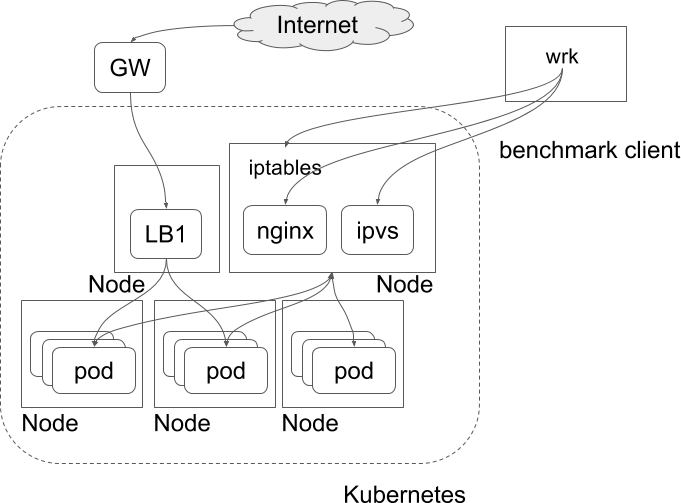
\includegraphics[width=0.8\columnwidth]{Figs/benchmark-schem}
  \caption[Benchmark setup]{Benchmark setup}
  \label{fig:lb_single_schem}
\end{figure}

\begin{table}[h]
  \centering
  \begin{tabular}{l}
    \hline
    \begin{minipage}{0.8\columnwidth}
      \begin{verbatim}

[Command line] 
 wrk -c800 -t40 -d30s http://172.16.72.2:8888/ 
-c: concurrency, -t: # of thread, -d: duration 

[Output example] 
 Running 30s test @ http://10.254.0.10:81/ 
  40 threads and 800 connections 
  Thread Stats   Avg      Stdev     Max   +/- Stdev 
    Latency    15.82ms   41.45ms   1.90s    91.90\% 
    Req/Sec     4.14k   342.26     6.45k    69.24\% 
  4958000 requests in 30.10s, 1.14GB read 
  Socket errors: connect 0, read 0, write 0, timeout 1 
Requests/sec: 164717.63 
Transfer/sec:     38.86MB 
      \end{verbatim}
    \end{minipage}
    \\ \hline
  \end{tabular}
  \caption[Benchmark command line and output example]{Benchmark command line and output example.}
  \label{tab:bench_example}
\end{table}

Fig.~\ref{fig:benchmark-schem}~(\subref{fig:bench_example}) shows an example of the command-line for wrk and the corresponding output.
The command-line in Fig.~\ref{fig:benchmark-schem}~(\subref{fig:bench_example}) will generate 40 wrk program threads
and allow those threads to send out a total of 800 concurrent HTTP requests over the period of 30 seconds.
The output example shows information including per-thread statistics, error counts, throughput in [Request/sec] and data rate in [Transfer/sec]

{
\setlength{\tabcolsep}{1em}
\renewcommand{\arraystretch}{1.2}

\begin{table}[tb]
  \centering
  \begin{tabular}{ll}
    \hline 
    \multicolumn{2}{l}{[Hardware Specification]}   \\
    & CPU: Xeon E5-2450 2.10GHz (with 8 core, Hyper Threading) \\
    & Memory: 32GB \\
    & NIC: Broadcom BCM5720 Giga bit \\
    & (Node x 6, Load Balacner x 1, Client x 1) \\
    & \\
    \multicolumn{2}{l}{[Node Software]}  \\
    & OS: Debian 8.7, linux-3.16.0-4-amd64 \\
    & Kubernetes v1.10.6 \\
    & flannel v0.7.0 \\
    & etcd version: 3.0.15 \\
    & \\
    \multicolumn{2}{l}{[Container Software]}   \\
    & Keepalived: v1.3.2 (12/03,2016) \\
    & nginx : 1.11.1(load balancer), 1.13.0(web server) \\
    \hline
  \end{tabular}
  \caption[Hardware and software specifications]{Hardware and software specifications.}
    \label{fig:hw_machine_spec}
\end{table}


\begin{table}[tb]
  \centering
  \begin{tabular}{ll}
    \hline 
    \multicolumn{2}{l}{[GCP VM Instance Specification]}   \\
    & Instance type: custom instance \\
    & CPU: Xeon 2.2GHz, 8, 16, 32 cpus \hspace{2cm} \\
    & Memory: 16GB \\
    & NIC: virtio\_net /w 16 rx-queues, 1Gbps \\
    & (Node x 6, Load balancer x 1, Client x 1) \\
    & \\
    \multicolumn{2}{l}{[AWS VM Instance Specification]}   \\
    & Instance type: c4.2xlarge, c4.4xlarge, c4.8xlarge  \\
    & CPU: Xeon E5-2666 v3 2.90GHz, 8, 16, 32 cpus \\
    & Memory: 64GB \\
    & NIC: ixgbevf /w 2 rx-queues, 1Gbps \\
    & (Node x 6, Load balancer x 1, Client x 1) \\
    \hline
  \end{tabular}
  \caption[Virtual Machine specifications]{Virtual Machine specifications.}
  \label{fig:cloud_machine_spec}
\end{table}
}

Fig.~\ref{fig:benchmark-spec}~(\subref{fig:machine_spec}) shows hardware and virtual machine specifications for experiments in on-premise data center and cloud environments.
We used a total of eight servers; six servers for Nodes, one for the load balancer and one for the benchmark client, with all having the same hardware specifications.
The software versions used for Kubernetes, web server and load balancer {\em pods} used in our experiments are also summarized in Fig.~\ref{fig:benchmark-spec}~(\subref{fig:software_spec}).

%\section{PHD}

\subsection{Effect of multicore proccessing}

Figure~\ref{fig:ipvs_mcore_proccessing} shows a result of throughput experiment with different multicore proccessing settings.
The following three RSS and RPS settings were compared: 
\begin{center}
  \centering
  \begin{minipage}{0.8\columnwidth}
\begin{verbatim}
(RSS, RPS) = (off, off)
           = (on , off)
           = (off, on )
\end{verbatim}
  \end{minipage}
\end{center}
%The host-gw mode of flannel backends is used as the overlay network.

\begin{figure}[h]
  \centering
  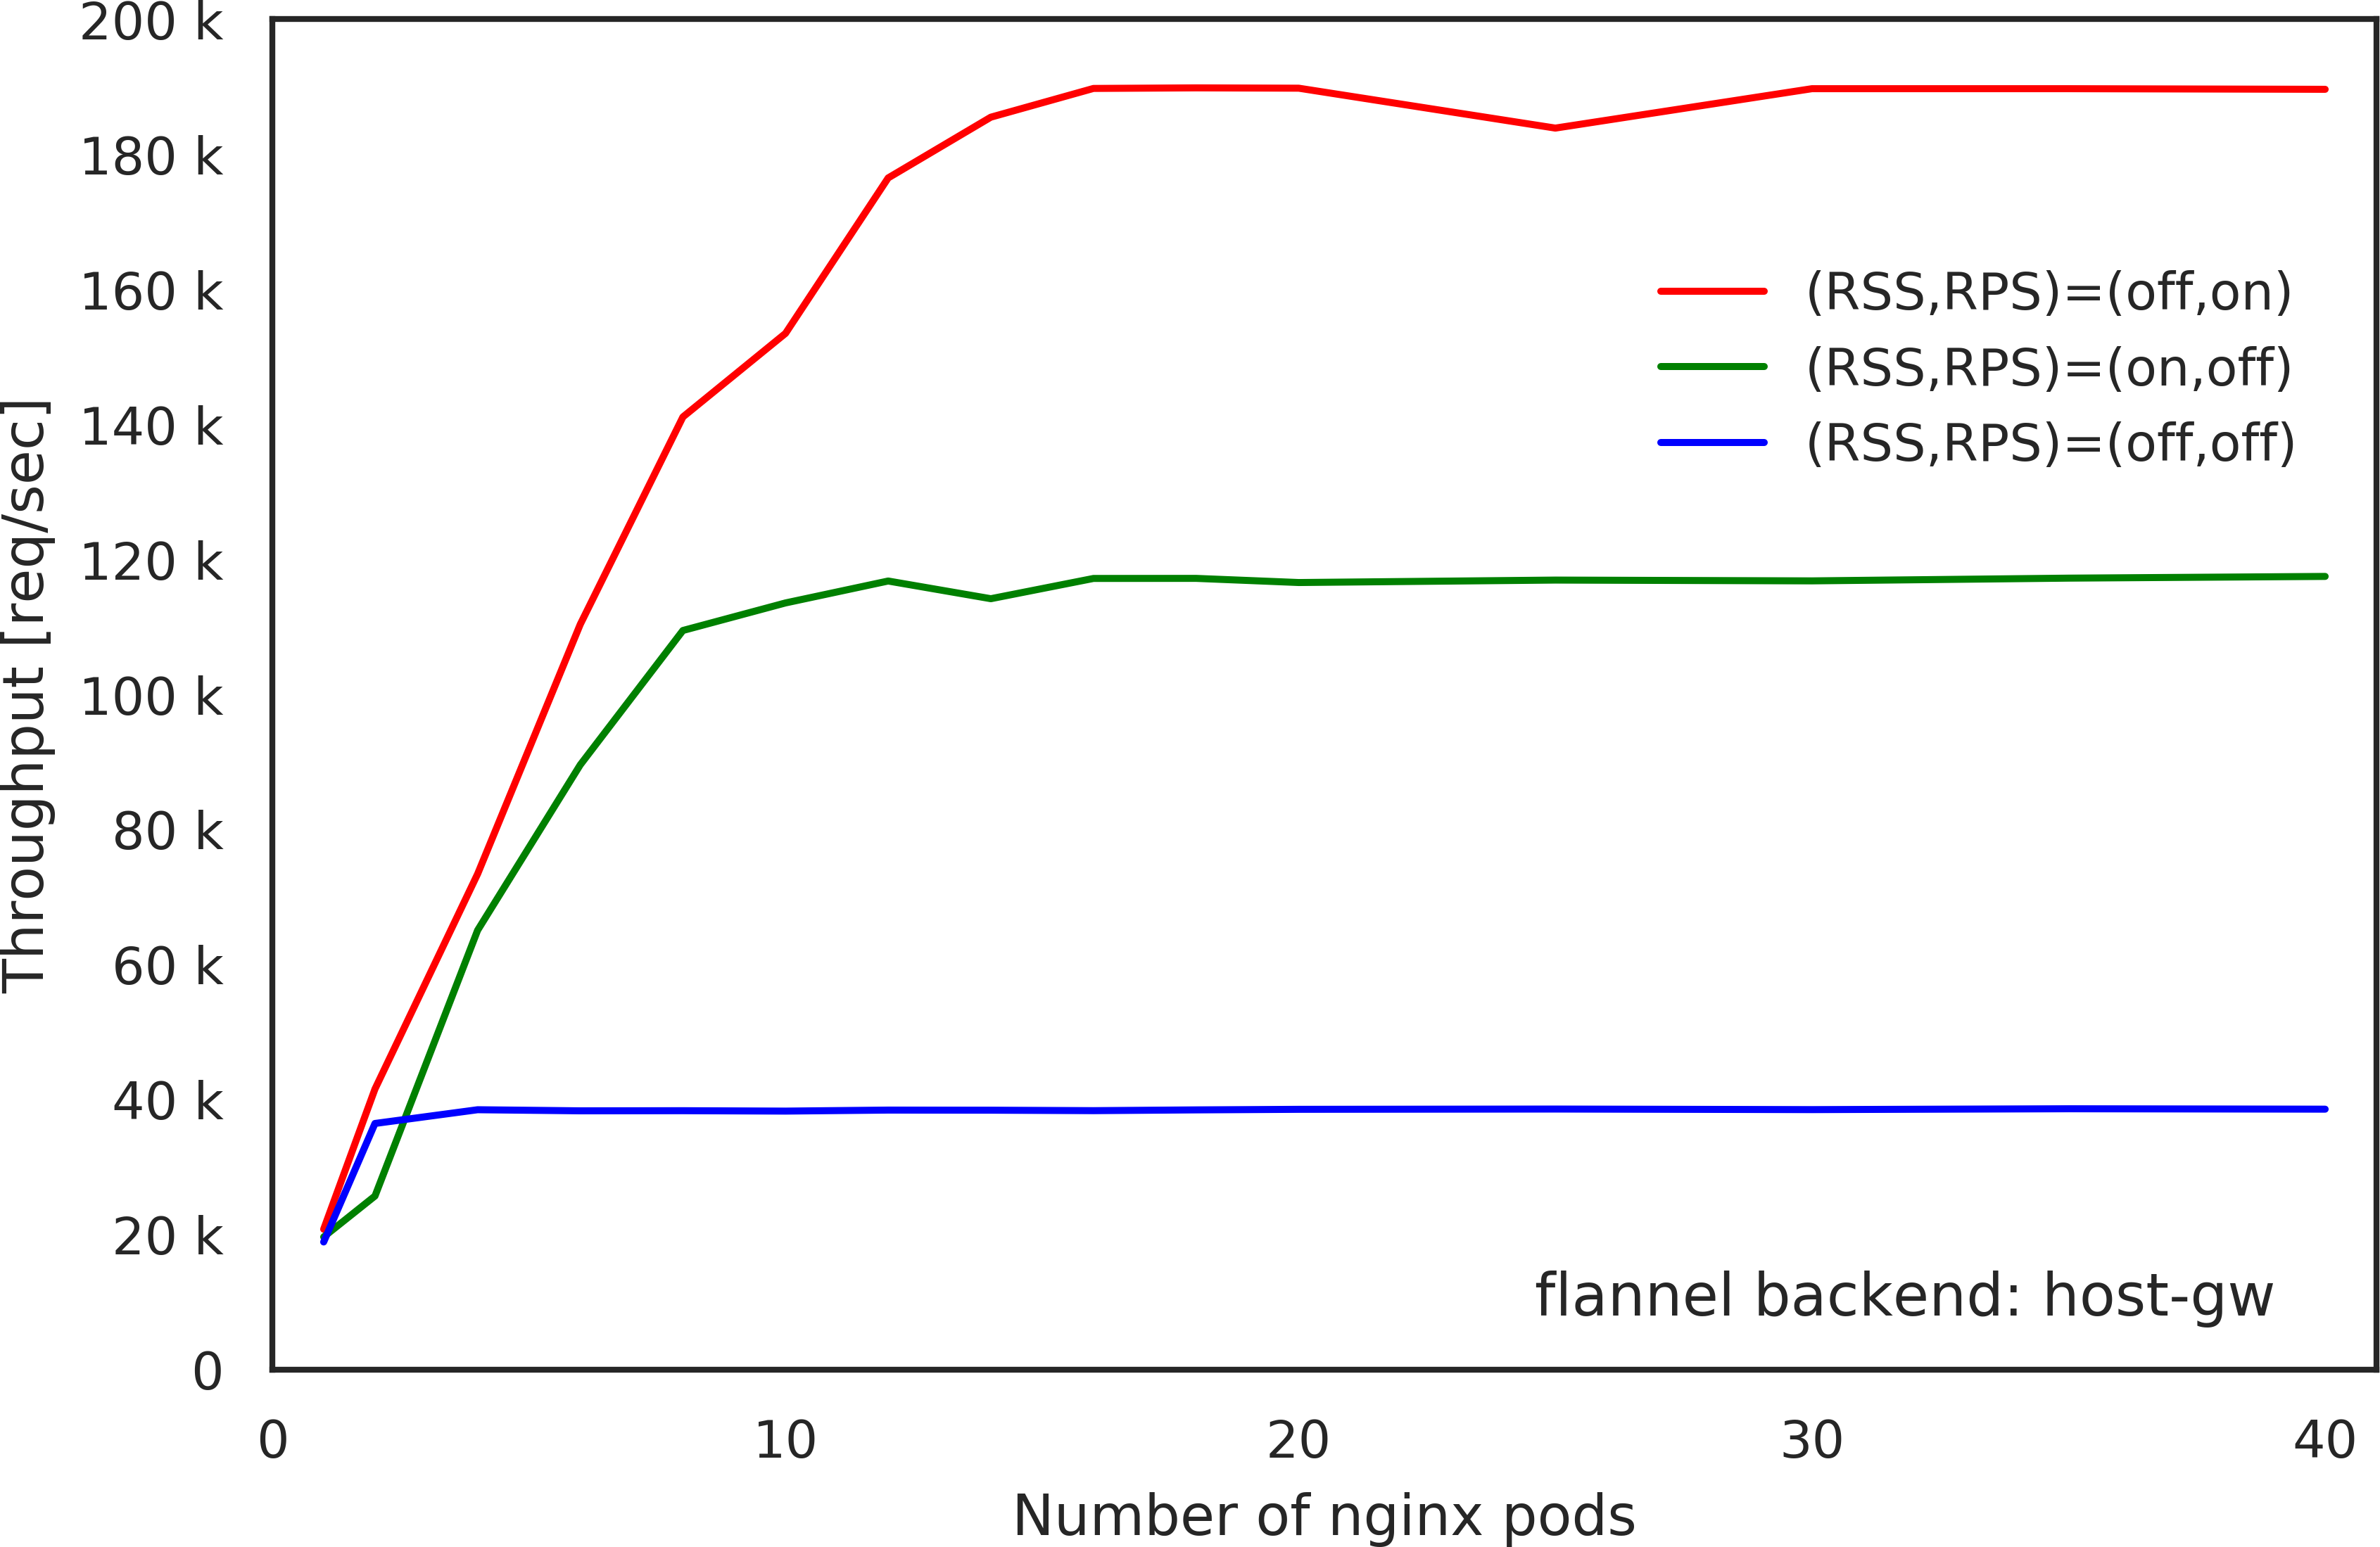
\includegraphics[width=0.8\columnwidth]{Figs/ipvs_mcore_proccessing}
  \caption{Effect of multicore proccessing on ipvs throughput.}
  \label{fig:ipvs_mcore_proccessing}
\end{figure}

The case with \enquote{(RSS, RPS) = (off, off)} means that multicore packet processing is completely disabled, i.e.,  all the incoming packets are processed by a single core.
The \enquote{(RSS, RPS) = (on, off)} means that the interrupt handling and the following IP protocol processing are performed on four of the CPU cores by assigning four rx-queues to those cores. In this case four of the eight CPU cores are utilized.
The \enquote{(RSS, RPS) = (off, on)} means that a single core handles all of the interrupts from the NIC then the following IP processings are performed on the other cores. In this case, all of the eight CPU cores are utilized.

We can see a general trend in which the throughput linearly increases as the number of nginx {\em pod}s increases and then it eventually saturates.
The saturated throughput levels indicate the maximum performance level of the ipvs load balancer.
The maximum performance levels depend on the (RSS, RPS) settings.
From the results in this figure, it can be seen that if we turn off multicore packet processing,
{\it i.e.}, when \enquote{(RSS, RPS) = (off, off)}, performance degrades significantly.
%In this case, the performance bottleneck is primarily due to packet processing in a single core.

If we compare the results for the cases when \enquote{(RSS, RPS) = (on, off)} and \enquote{(RSS, RPS) = (off, on)},
the latter is better than the former.
It is clear that the case that utilizes all of the CPU cores better performs than the case with only four CPU cores utilized. 

\FloatBarrier

\subsection{Effect of overlay network}

\begin{figure}[h]
  \centering
  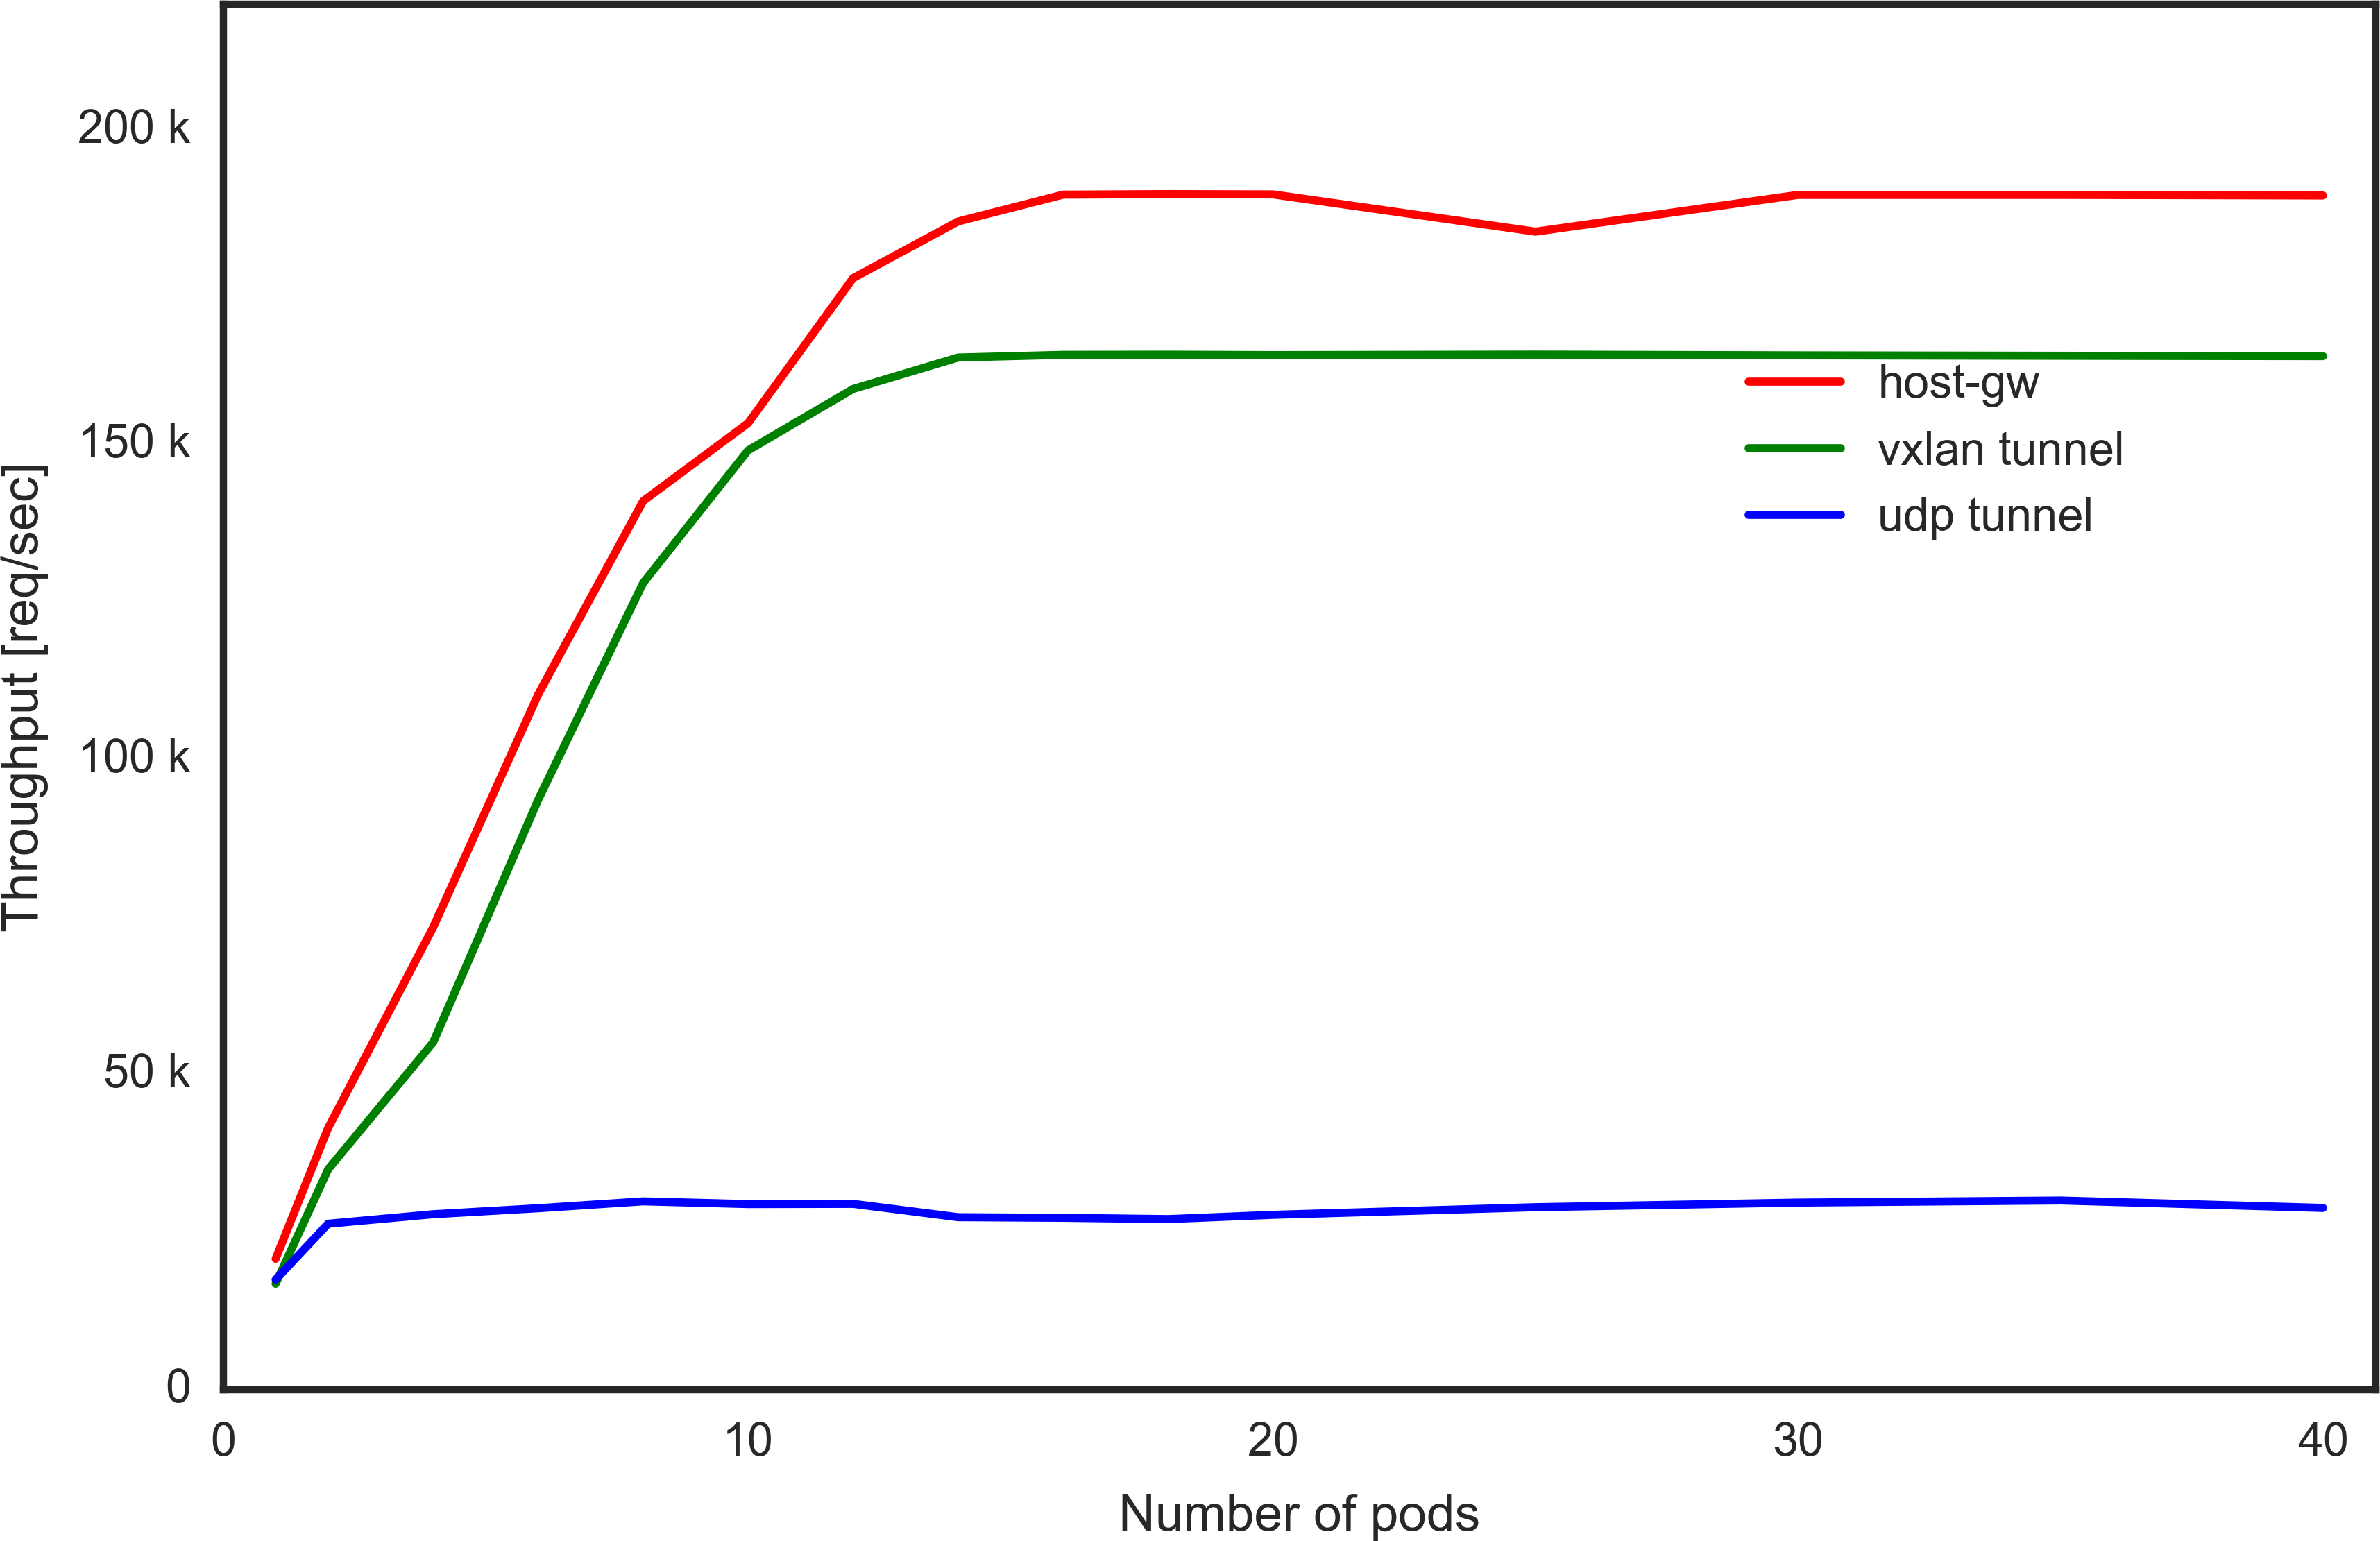
\includegraphics[width=0.8\columnwidth]{Figs/ipvs_flannel_mode}
  \caption{Effect of flannel backend modes on ipvs throughput.}
  \label{fig:ipvs_flannel_mode}
\end{figure}

Figure~\ref{fig:ipvs_flannel_mode} shows the ipvs throughput results for different overlay network settings.
As for the overlay network, the author used the flannel and measured the performance levels for flannel's three backend modes, host-gw, vxlan and udp.
Except for the udp backend mode case, we can see the trend in which the throughput linearly increases as the number of nginx {\em pod} increases and then it eventually saturates.
The saturated throughput levels indicate the maximum performance levels of the ipvs load balancer.
If we compare the performance levels among the flannel backend modes types, 
the host-gw mode where no encapsulation is conducted shows the highest performance level,
followed by the vxlan mode where the Linux kernel encapsulate the Ethernet frame.
The udp mode where flanneld itself encapsulate the IP packet shows significantly lower performances levels.
The author considers the host-gw mode is the best, the vxlan tunnel the second best and the udp tunnel mode unusable.
As is shown here, overlay network settings greately affect the performance level.
The author used host-gw mode for most of the experiments conducted in on-premise data centers and vxlan mode for the experiments conducted in cloud environments.  

\FloatBarrier

\subsection{Comparison of different load balancer}

\begin{figure}[h]
  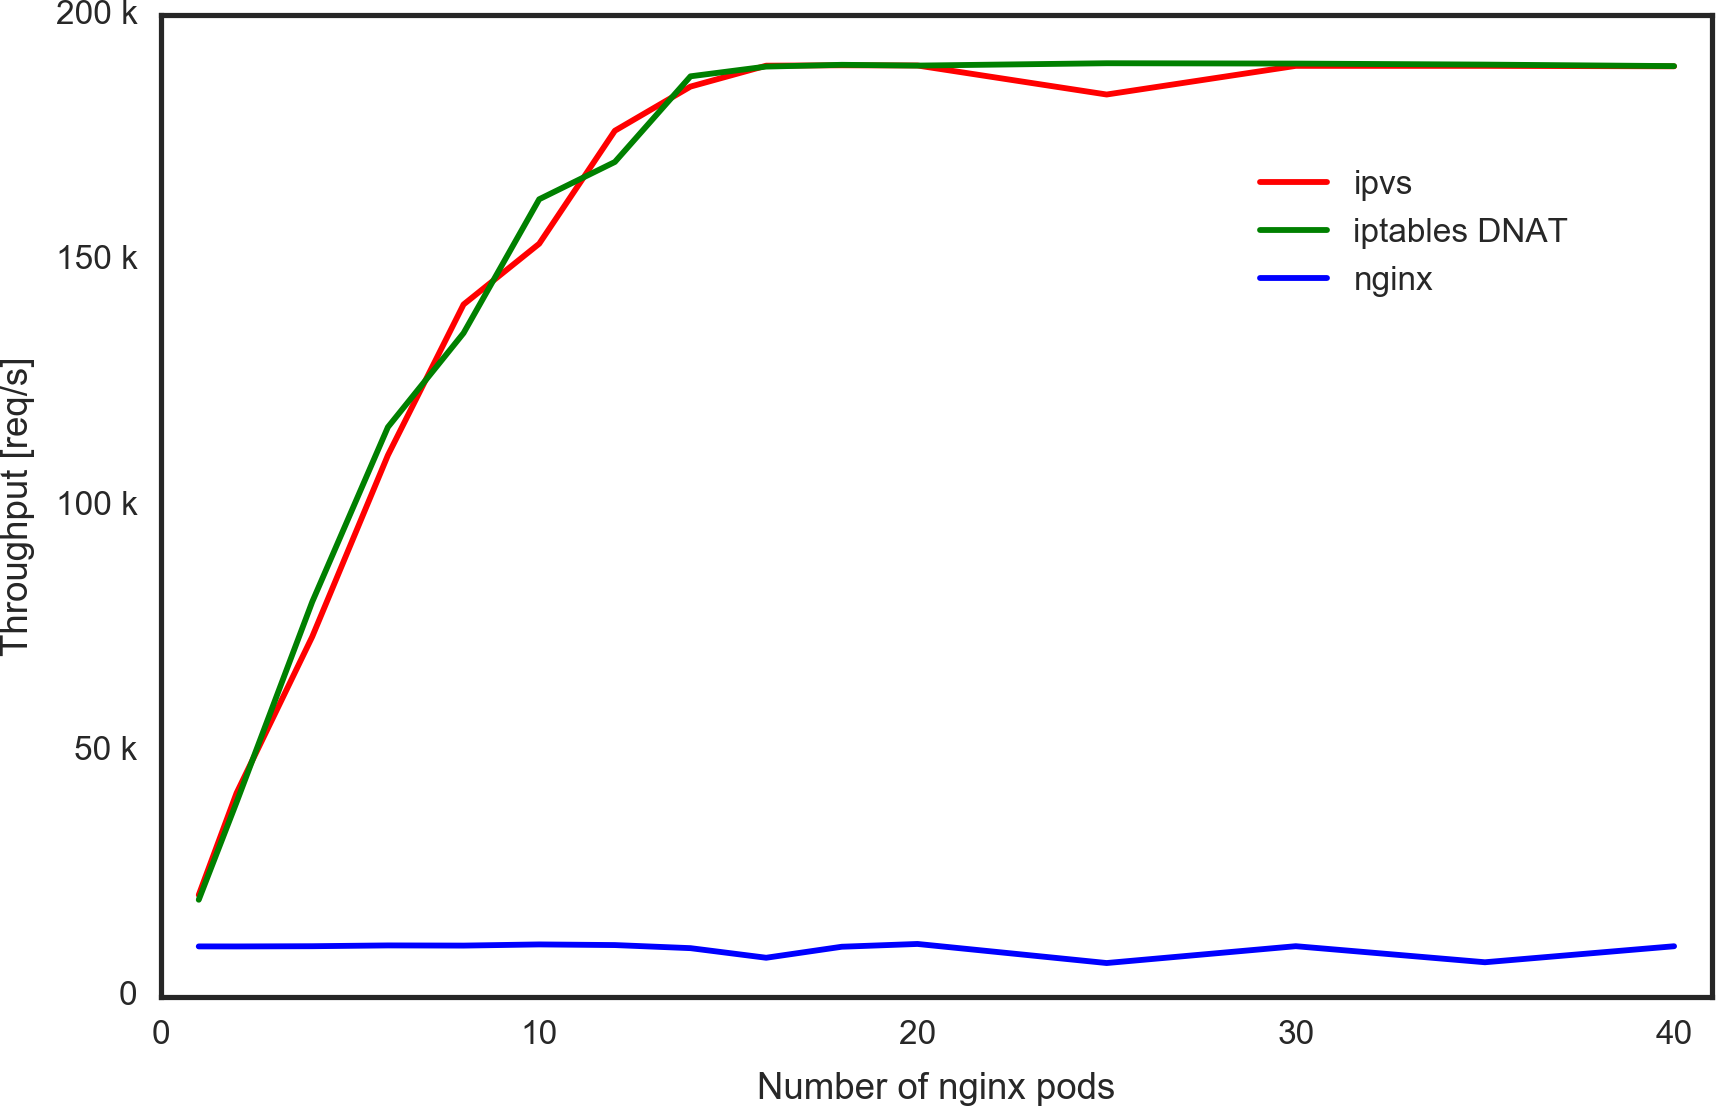
\includegraphics[width=0.9\columnwidth]{Figs/ipvs-iptables-nginx}
  \caption{Throughput measurement results of the proposed load balancer in on-premise data center.}
  \label{fig:ipvs-iptables-nginx}
\end{figure}

\interfootnotelinepenalty=10000

Fig.~\ref{fig:ipvs_performance}~(\subref{fig:ipvs-iptables-nginx}) shows the throughput of the proposed ipvs container load balancer.
The performance of the nginx and the iptables DNAT as the load balancers are also presented for comparison.
As we increased the number of the nginx pods(web servers) from 1 to around 14, the throughput increased almost linearly and after which it saturated.
The increase indicates that the load balancer functions properly because it increased throughput by distributing HTTP requests to multiple of the web servers.
The saturated performance level indicates the maximum performance of the load balancer, which could be determined either by network bandwidth or CPU performance level of the load balancer or the benchmark client.
In this specific experiment, the performance level was limited by the 1 Gbps bandwidth of experimental network\cite{takahashi2018portable}, which is revealed by packet level analysis using tcpdump.
On average the data size of each request and the corresponding response was about 636 [byte/req] in total, including TCP/IP headers, Ethernet header, and inter frame gaps.
Multiplying that with 190K [req/sec] and 8 [bit/byte] will result in 966.72 Mbps.

While nginx did not show any benefit as the load balancer, the performance of the ipvs load balancer container showed equivalent performance level as the un-containerized iptables DNAT.
This means that our proposed ipvs container load balancer is at least as good as the un-containerized iptables' load balancing in the 1 Gbps network.

\subsection{Comparison of different load balancer}

\begin{figure}[h]
  \centering
  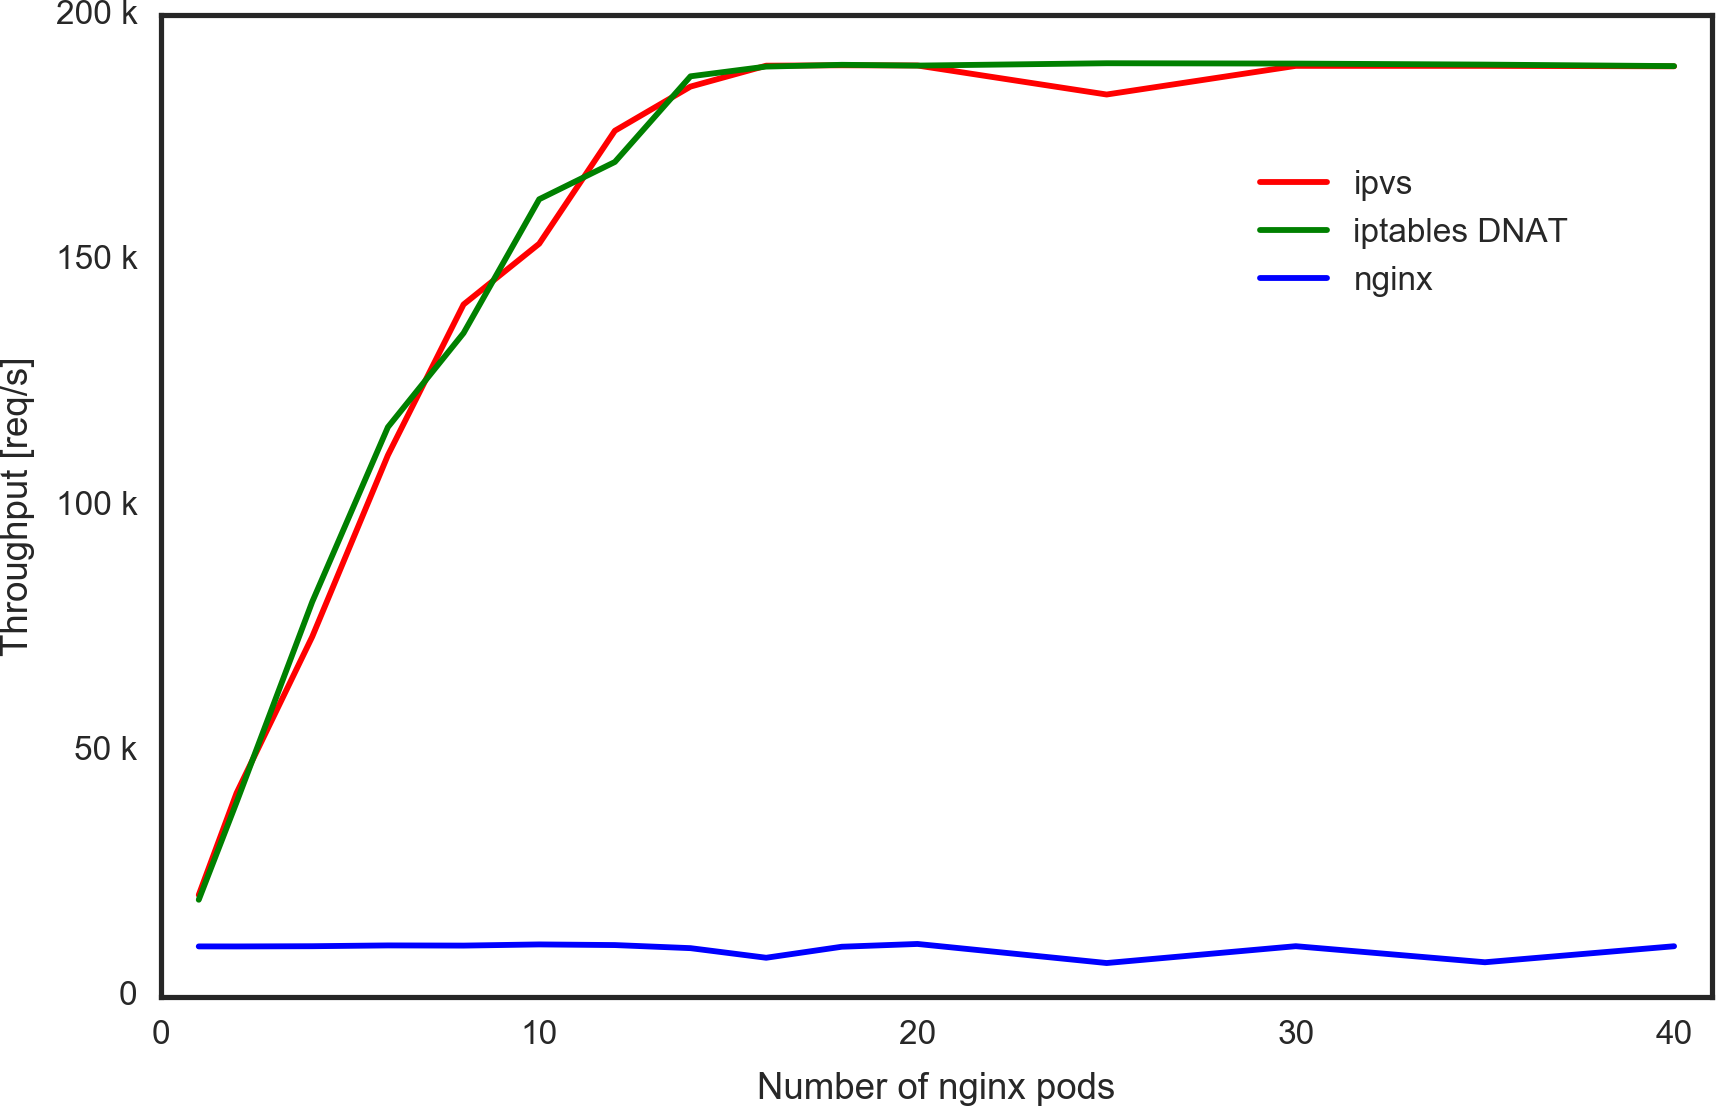
\includegraphics[width=0.8\columnwidth]{Figs/ipvs-iptables-nginx}
  \caption{Throughput comparison between ipvs, iptables DNAT and nginx.}
  \label{fig:ipvs-iptables-nginx}
\end{figure}

Figure~\ref{fig:ipvs-iptables-nginx} compares the performance measurement results for different load balancer ipvs, iptables DNAT, and nginx.
The proposed ipvs load balancer exhibits almost equivalent performance levels as the iptables DNAT based load balancer. 
The nginx based load balancer shows no performance improvement even though the number of the nginx web server {\em pods} is increased.
It is understandable because the performance of the single nginx as a load balancer is expected to be similar to the performance as a web server.

\begin{figure}[h]
  \centering
  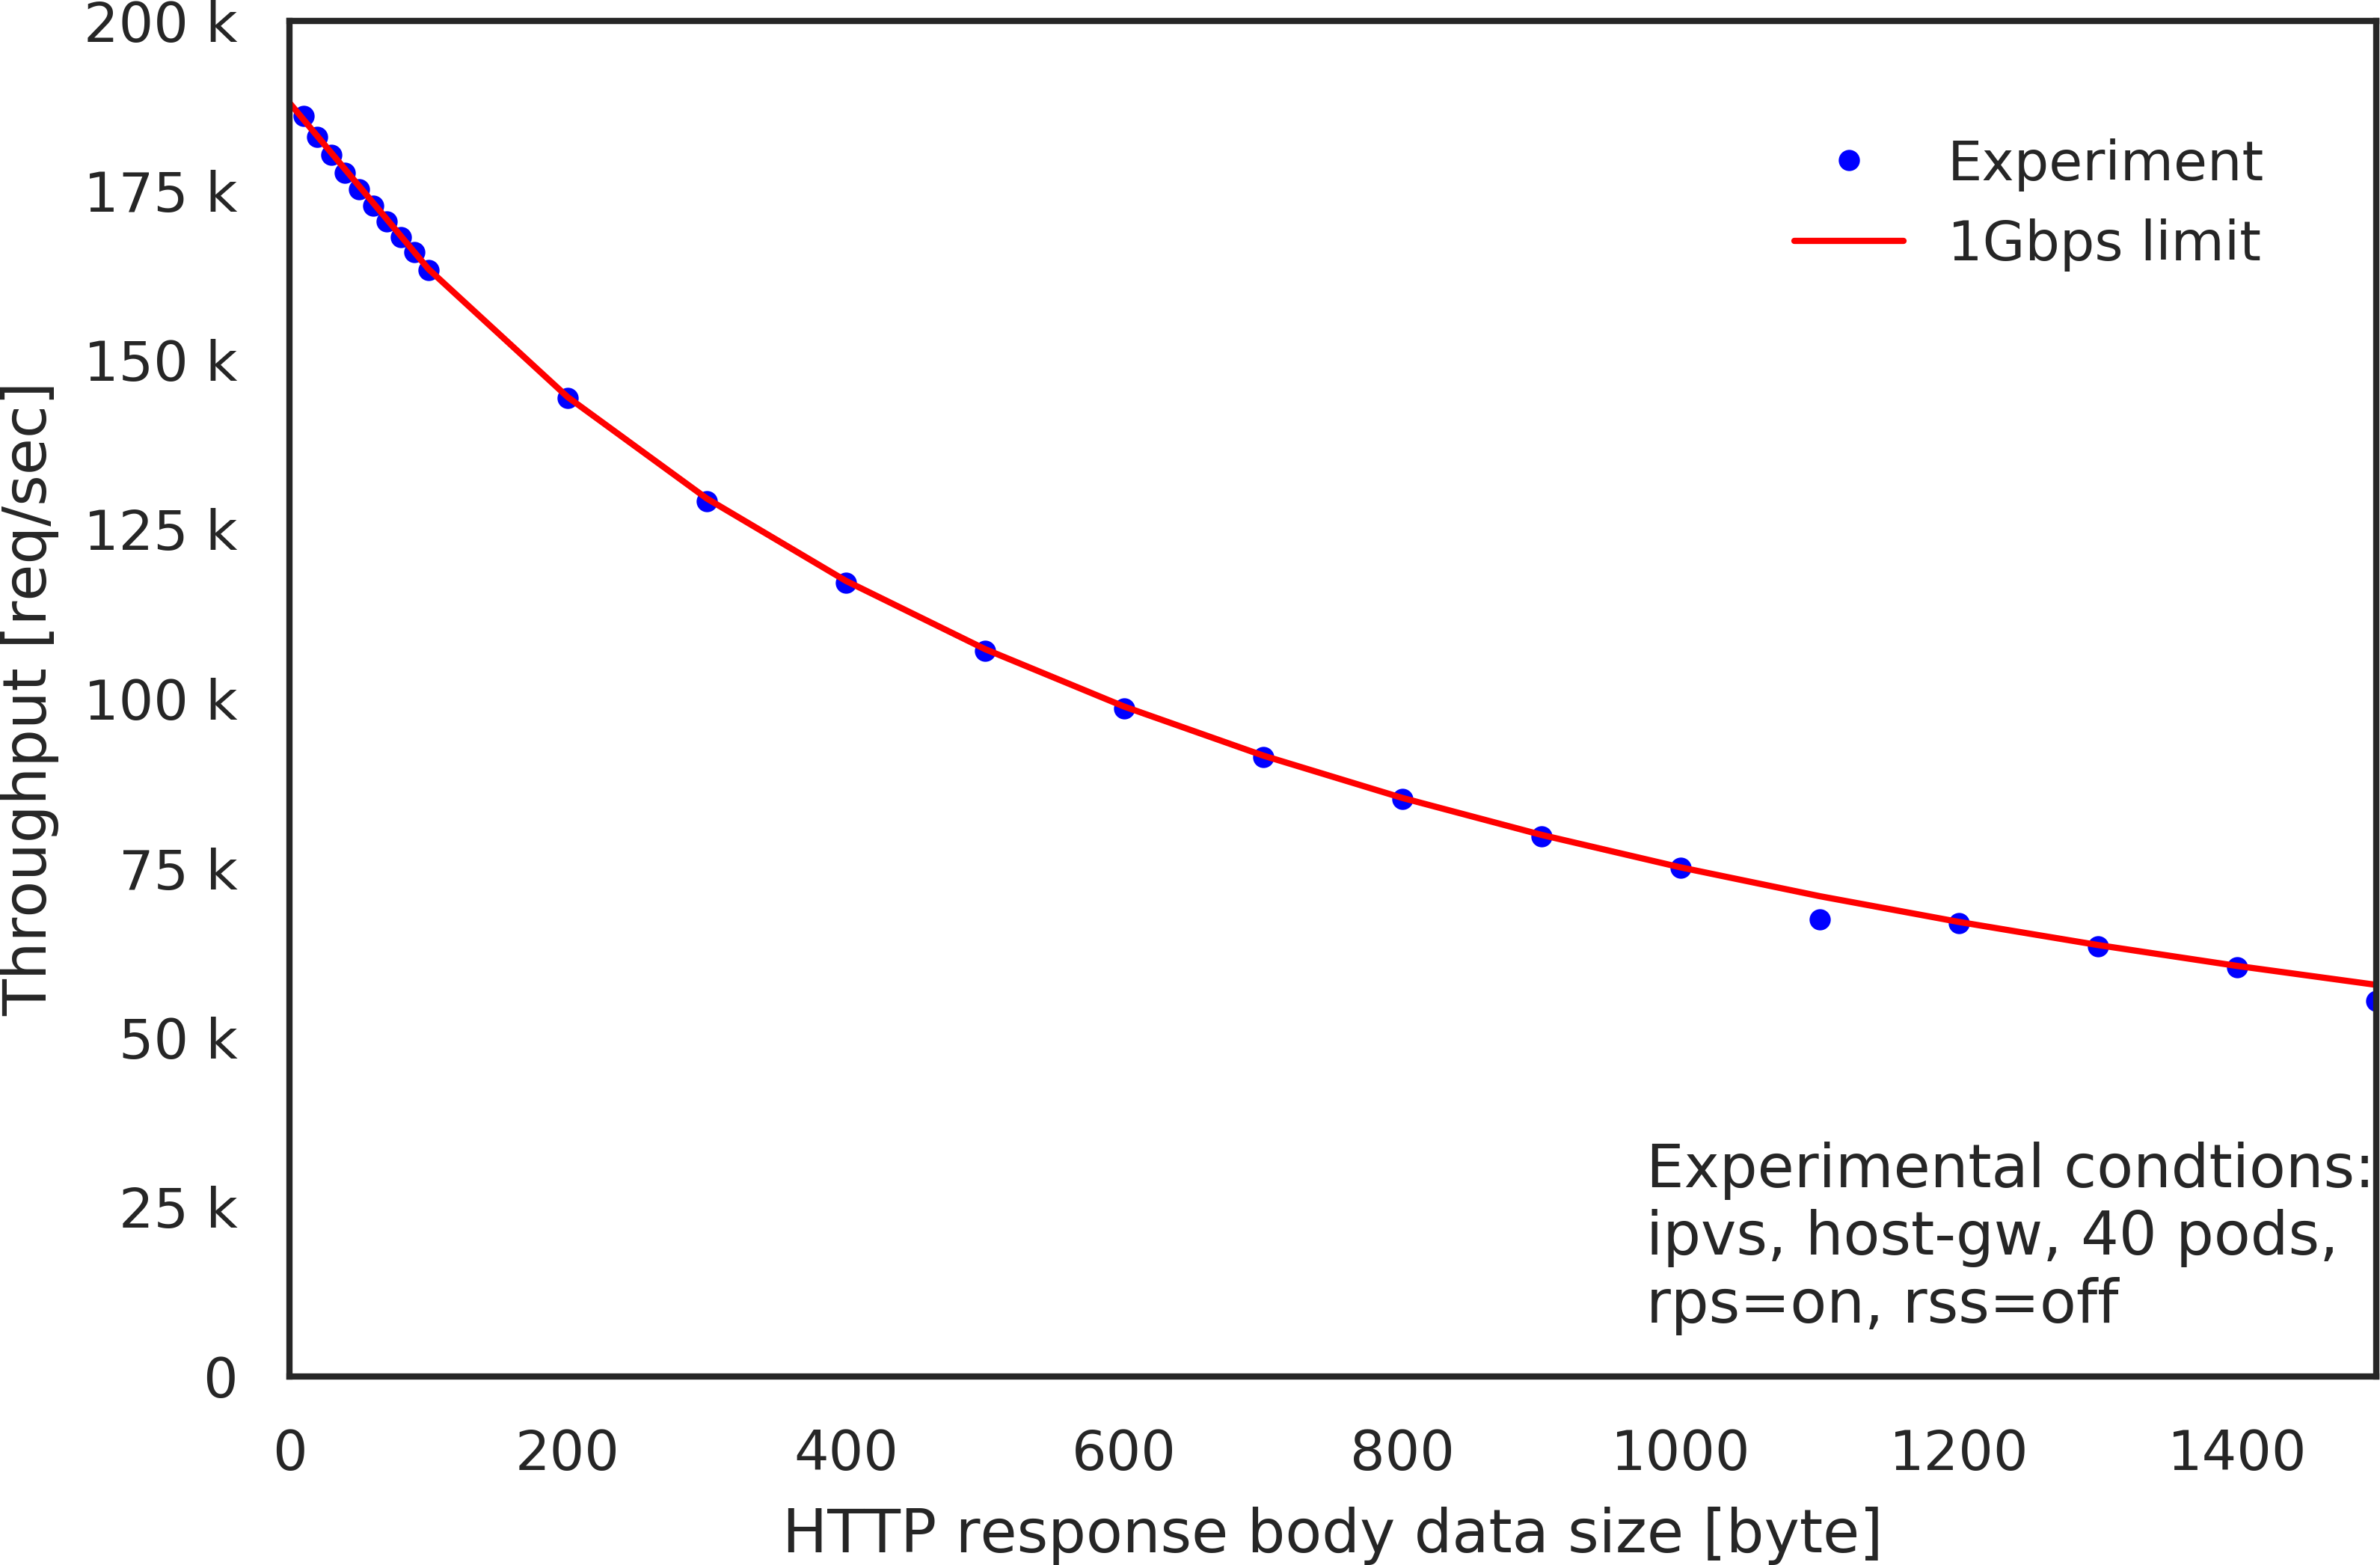
\includegraphics[width=0.8\columnwidth]{Figs/tp_limit_1gbps}
  \caption{Performance limit due to 1Gbps bandwidth}
  \label{fig:performance_limit}
\end{figure}

At first, it was not clear what caused the performance limit for the case when \enquote{(RSS, RPS) = (off, on)},
the author thought it was due to the insufficient CPU performance.
However, that was not the case in the conditions of the experiment; it turned out to be due to the 1Gbps bandwidth.
A packet level analysis using tcpdump\cite{jacobson1989tcpdump} revealed that 665.36 bytes of extra HTTP headers,
TCP/IP headers and ethernet frame headers are needed for each request in the case of the wrk benchmark program(Appendix~\ref{appendix:performance_limit}).
This results in the upper limit of 184,267 [req/sec] when the date size of HTTP response body is 13 byte, which agrees well with the performance limit for the case when \enquote{(RSS, RPS) = (off, on)} in Figure~\ref{fig:ipvs_mcore_proccessing}.
Figure~\ref{fig:performance_limit} shows the theoretical upper limit of the performance level for 1Gbps ethernet together with actual benchmark results for the range of larger data sizes, and they agree very well.
Therefore it can be said that when \enquote{RPS = on}, ipvs performance is limited by 1Gbps bandwidth.
The author regarded that \enquote{(RSS, RPS) = (off, on)} is the best setting in our experimental conditions, and used this setting throughout this thesis unless explicitly stated otherwise.

\begin{figure}[h]
  \centering
  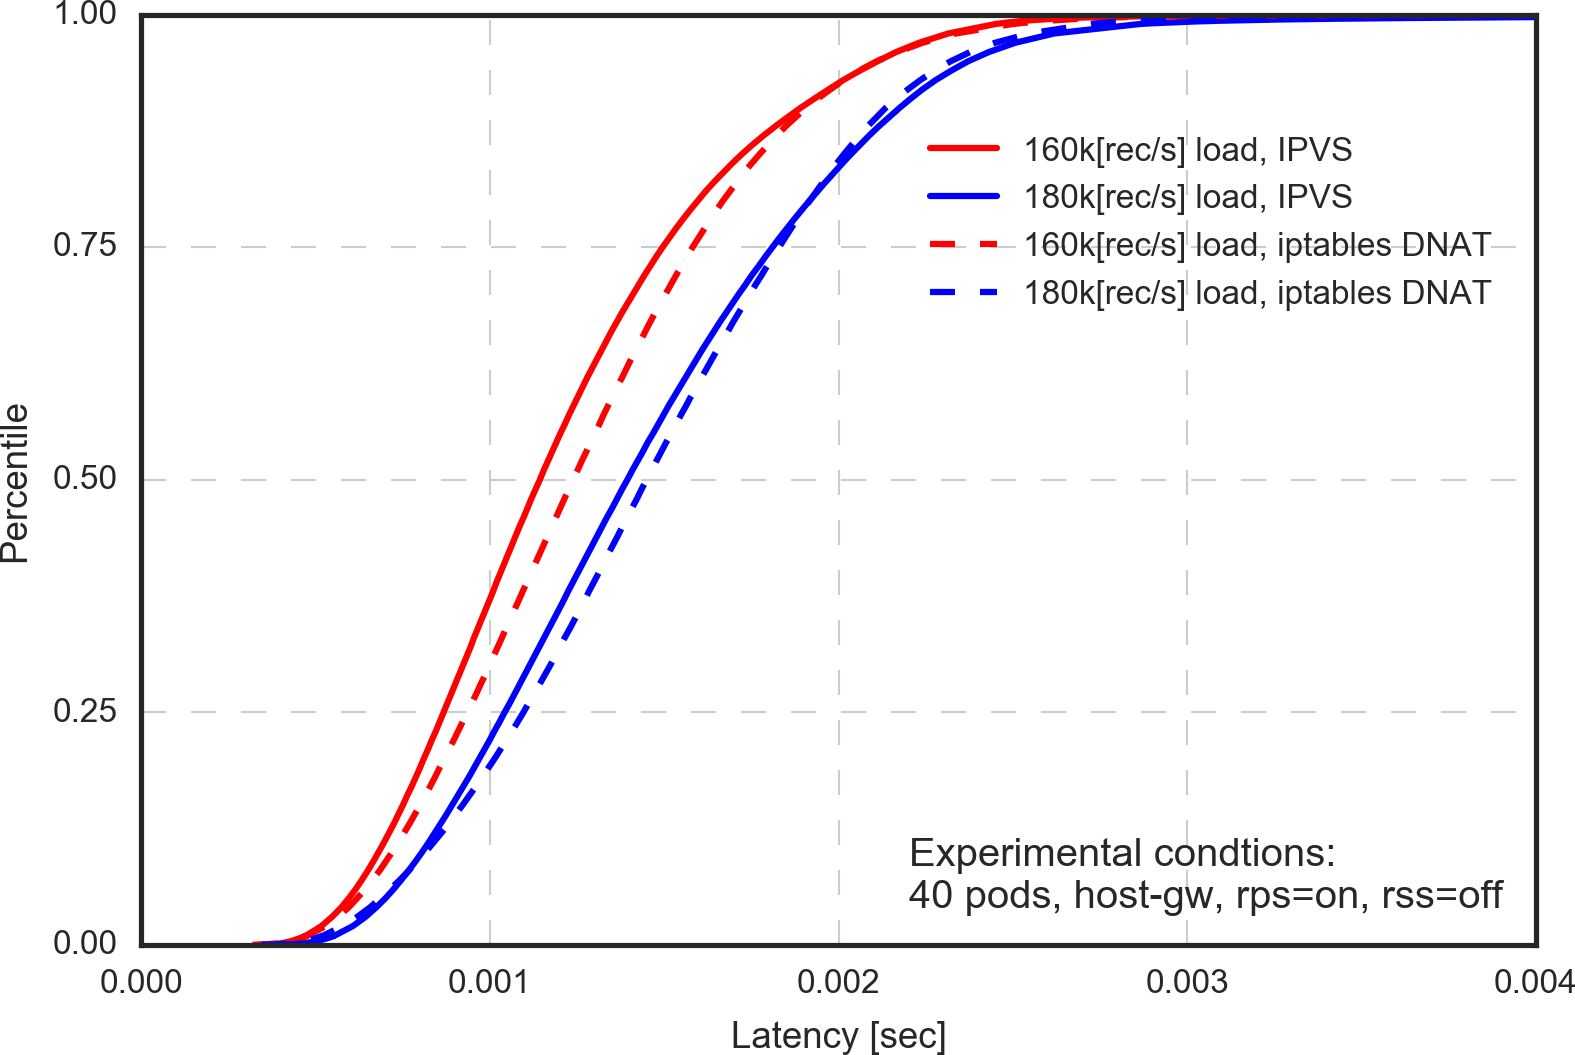
\includegraphics[width=0.8\columnwidth]{Figs/latency_cdf_rps_40pods}
  \caption{Latency cumulative distribution function.}
  \label{fig:latency_cdf_rps_40pods}
\end{figure}

Figure~\ref{fig:latency_cdf_rps_40pods} compares Cumulative Distribution Function(CDF) of the load balancer latency at the two constant loads, 160K[req/sec] and 180K[req/sec] for ipvs and iptables DNAT.
We can see that the latencies are a little bit smaller for ipvs.
For example, the median values at 160K[req/sec] load for ipvs and iptables DNAT are, 1.14 msec and 1.24 msec, respectively.
Also, at 160K[req/sec], they are 1.39 msec and 1.45 msec, respectively.
These may not be considered a significant difference; however, we can at least say that our proposed load balancer is as good as iptables DNAT.
So, to conclude this section, the containerized ipvs load balancer showed equivalent performance levels with the iptables DNAT load-balancing function that is used in Kubernetes cluster.

%\subsection{Resource Consumption}

Fig.~\ref{fig:cpu_usage} compares the CPU usage for proposed load balancer(ipvs in a container) and iptables DNAT at the time of the throughput measurement in the on-premise data center.
Since the CPU usage was higher for the ipvs in a container, the proposed load balancer may be less efficient compared with the iptables DNAT.
%The proposed architecture requires additional computational resources compared with the conventional architecture.
However since single hardware can accommodate 1 Gbps traffic with CPU usage of about 60\%, the authors regard this as a tolerable overhead.
The authors plan to improve the efficiency of the proposed load balancer by developing a software load balancer using eXpress data path(XDP) technology\cite{hoiland2018express} in the future work and thereby improving the performance levels of the portable load balancer.

\begin{figure}[h]
  \centering
  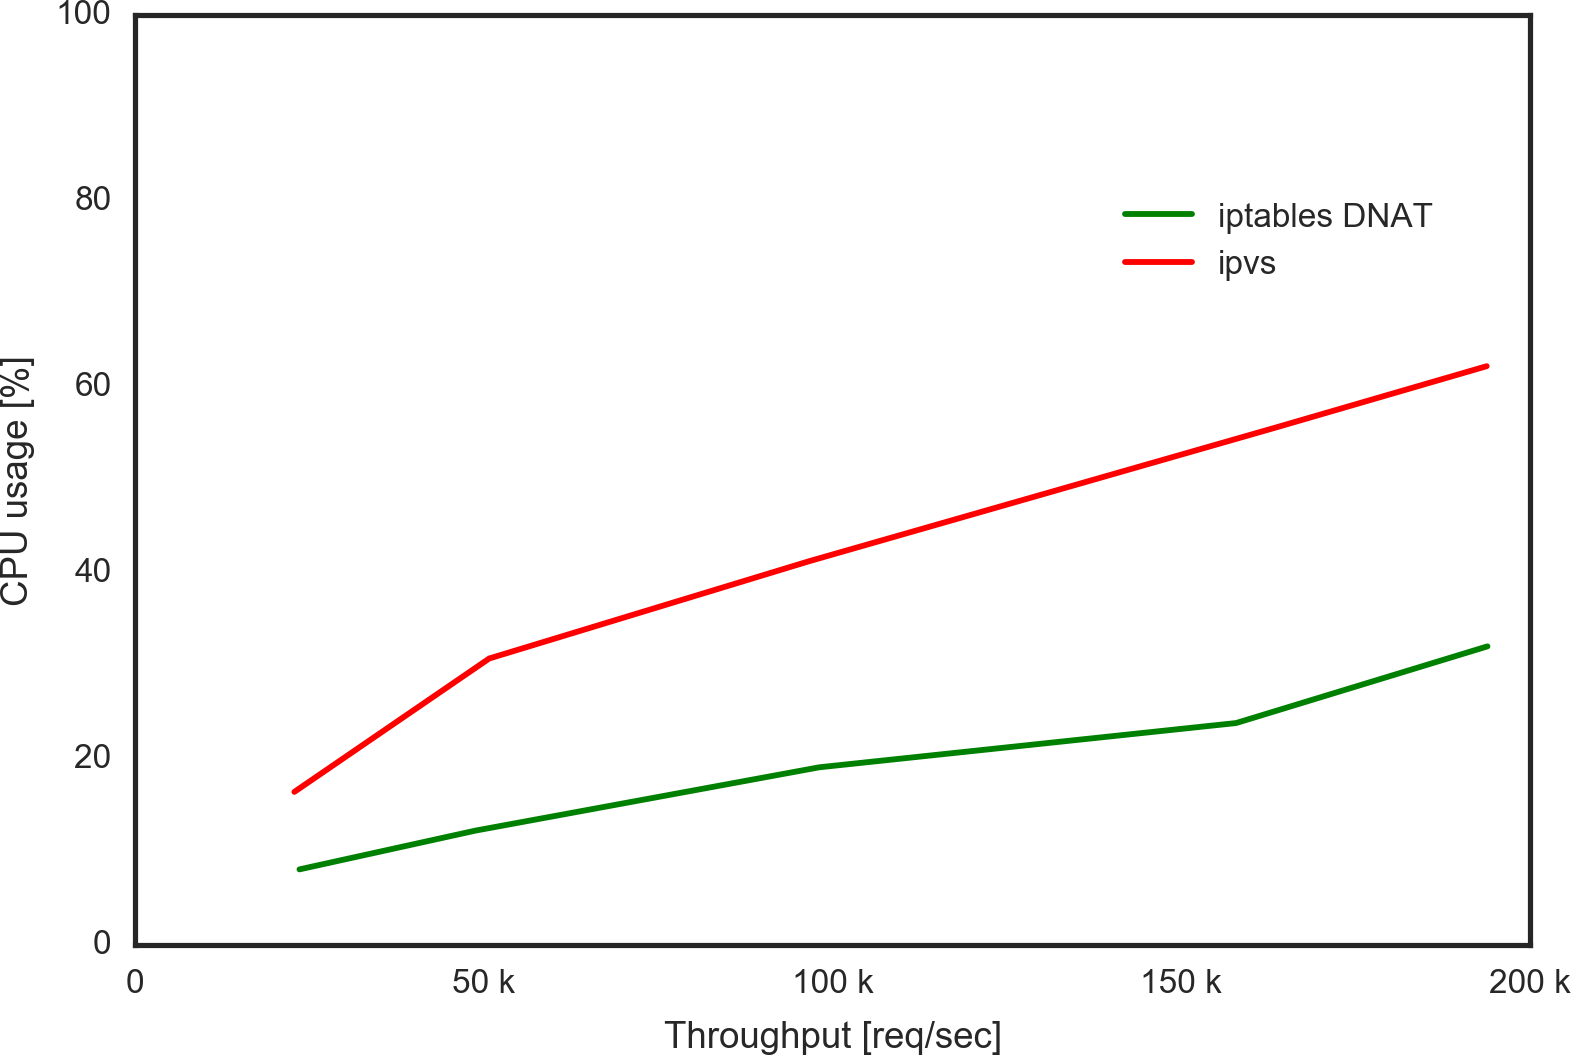
\includegraphics[width=0.8\columnwidth]{Figs/cpu_usage}
  \caption{CPU usage of the ipvs and iptables DNAT.}
  \label{fig:cpu_usage}
\end{figure}


\FloatBarrier

\subsection{L3DSR using ipvs tun}

The performance levels of ipvs and iptables DNAT have been limited by 1 Gbps bandwidth.
This can be alleviated in the case of ipvs by using so-called Layer 3 Direct Server Return(l3dsr) setup.
Figure~\ref{fig:bench_1g_l3dsr} shows the schematic diagram illustrating packet flow for the HTTP request packet(the red arrows) and response packet(the blue arrow).

\begin{figure}[h]
  \centering
  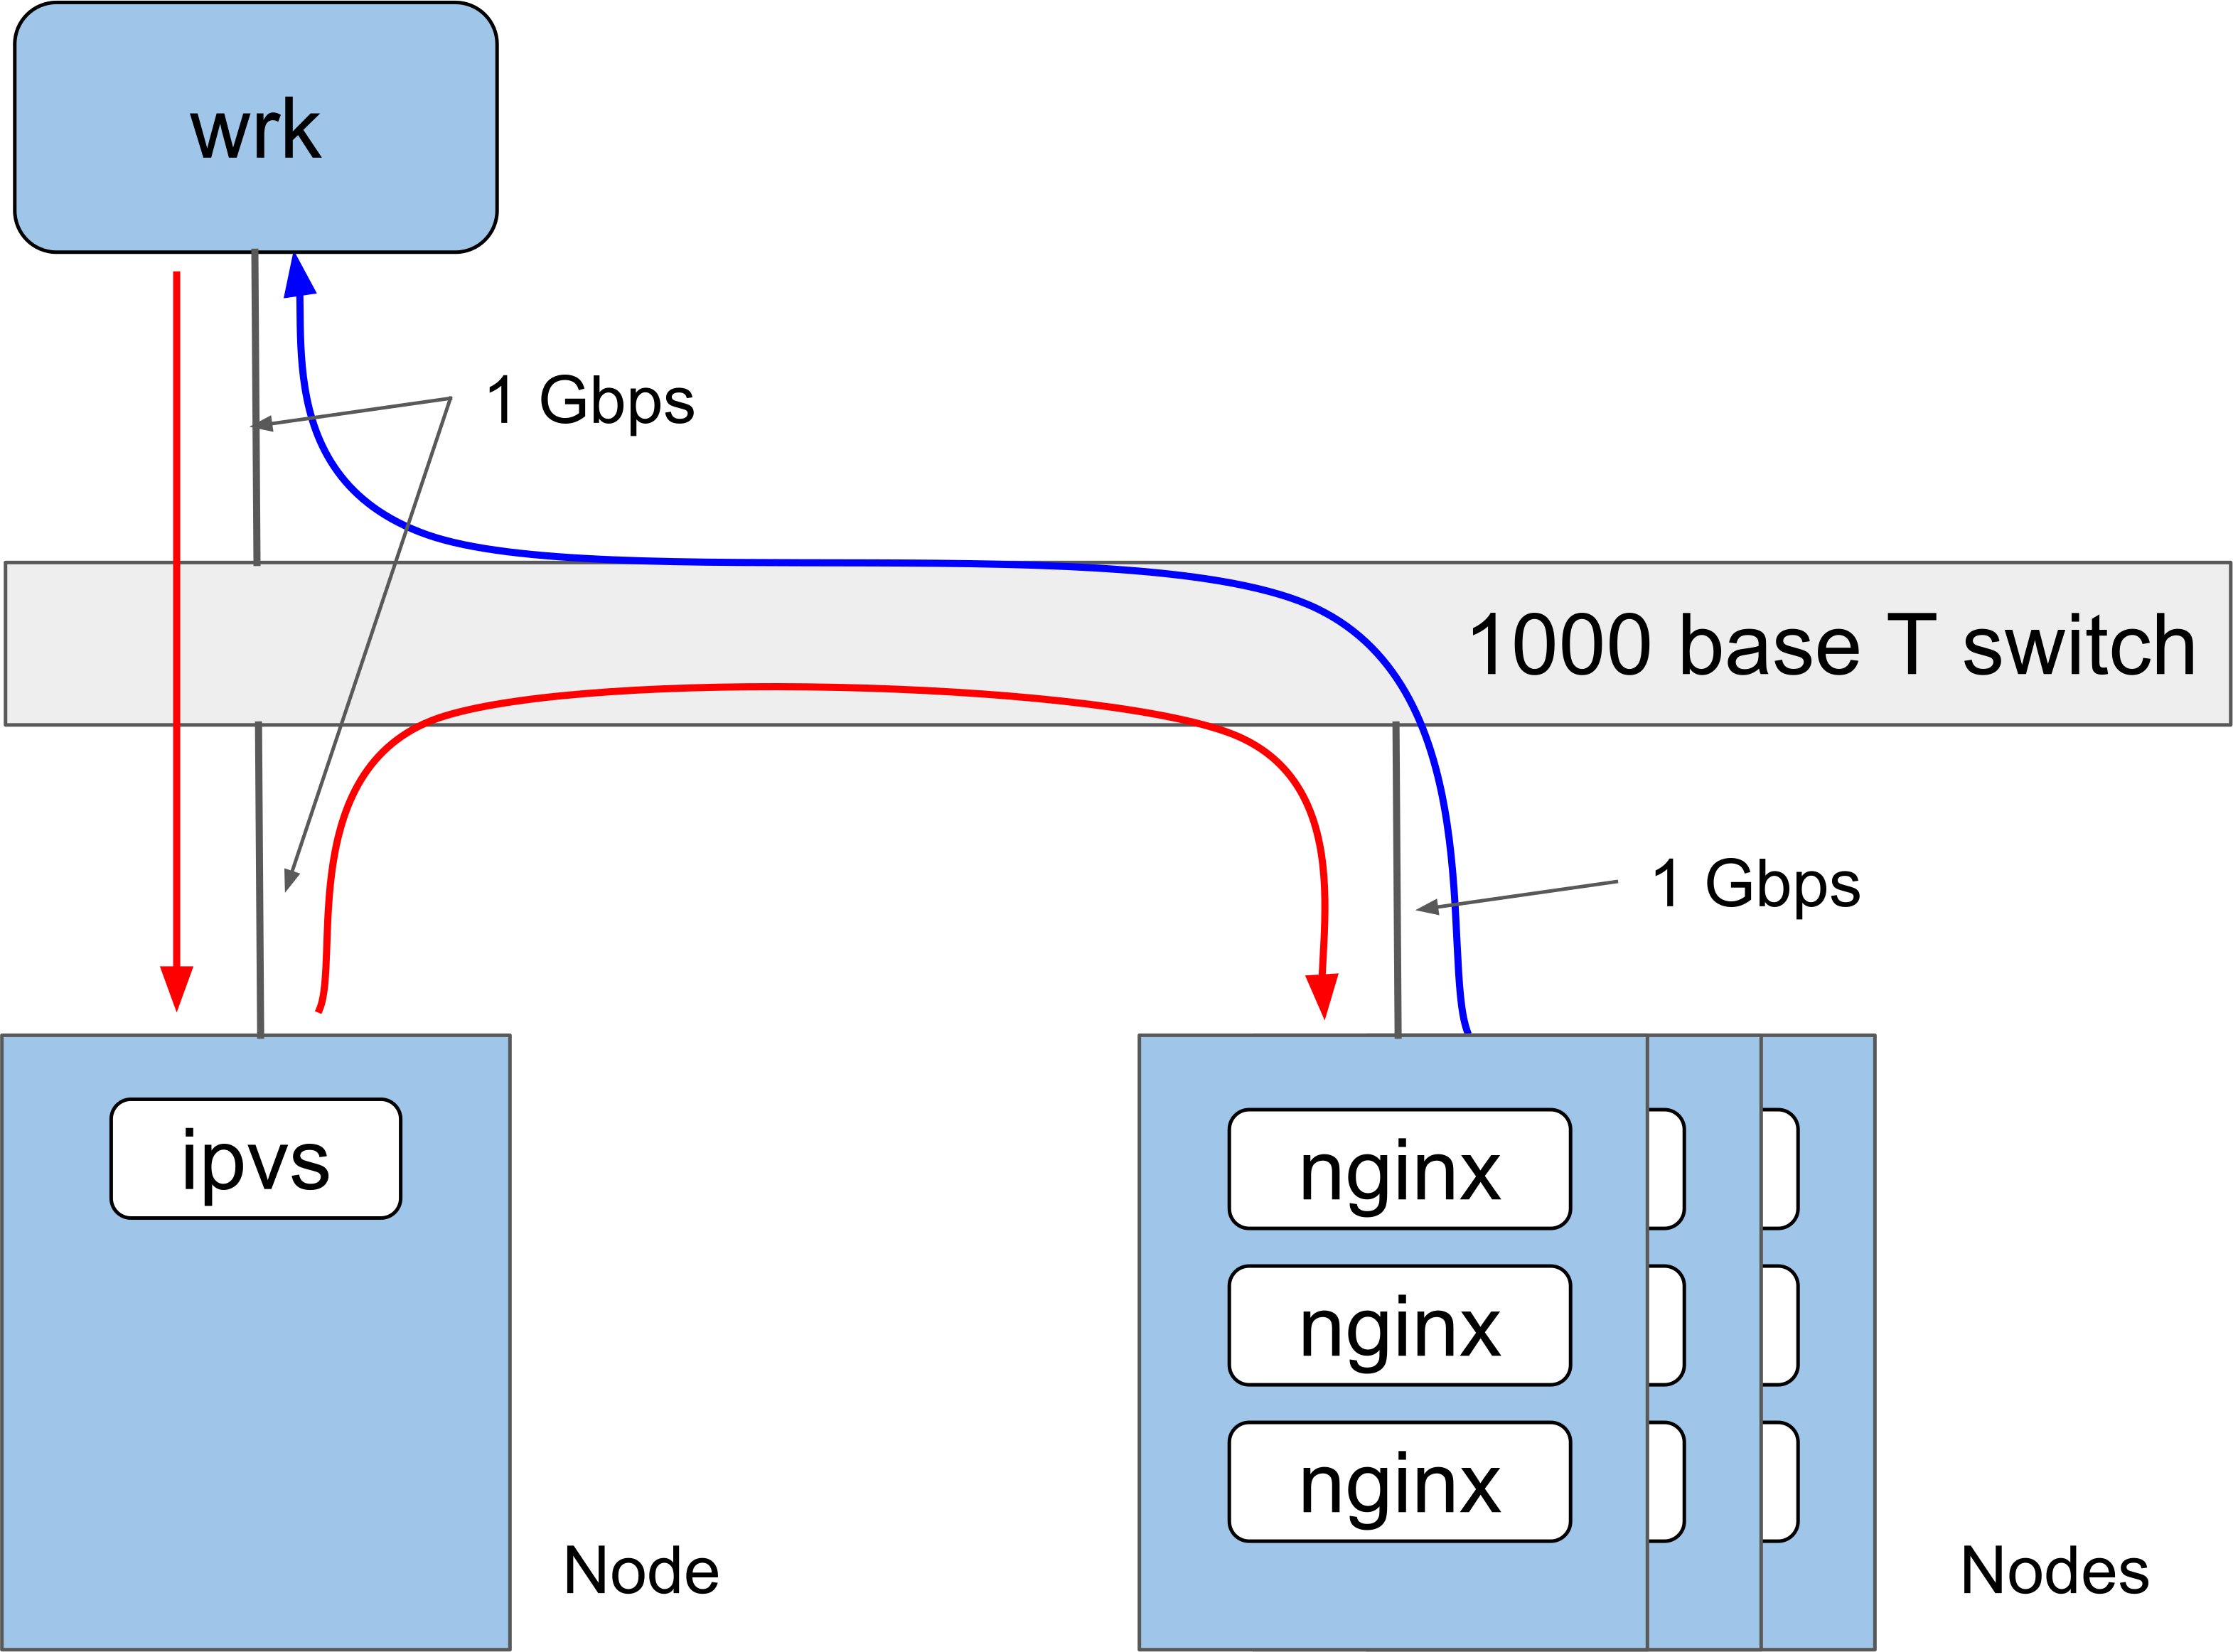
\includegraphics[width=0.8\columnwidth]{Figs/bench_1g_l3dsr}
  \caption{Physical configuration for L3DSR experiment.}
  \label{fig:bench_1g_l3dsr}
\end{figure}

The ipvs has the mode called ipvs-tun.
When the ipvs-tun send out the packets to real servers, it encapsulates the original packet in ipip tunneling packet that is destined to real servers.
The real server receives the packet on a tunl0 device and decapsulates the ipip packet, revealing the original packet.
Since the source IP address of the original packet is maintained, the returning packets are sent directly toward the benchmark client.
In this scheme, the returning packets do not consume the bandwidth nor the CPU power of the load balancer node.

The iptables DNAT does not have the functions that enable L3DSR settings.
Therefore this one of the benefits of the ipvs load balancer.

\begin{figure}[h]
  \centering
  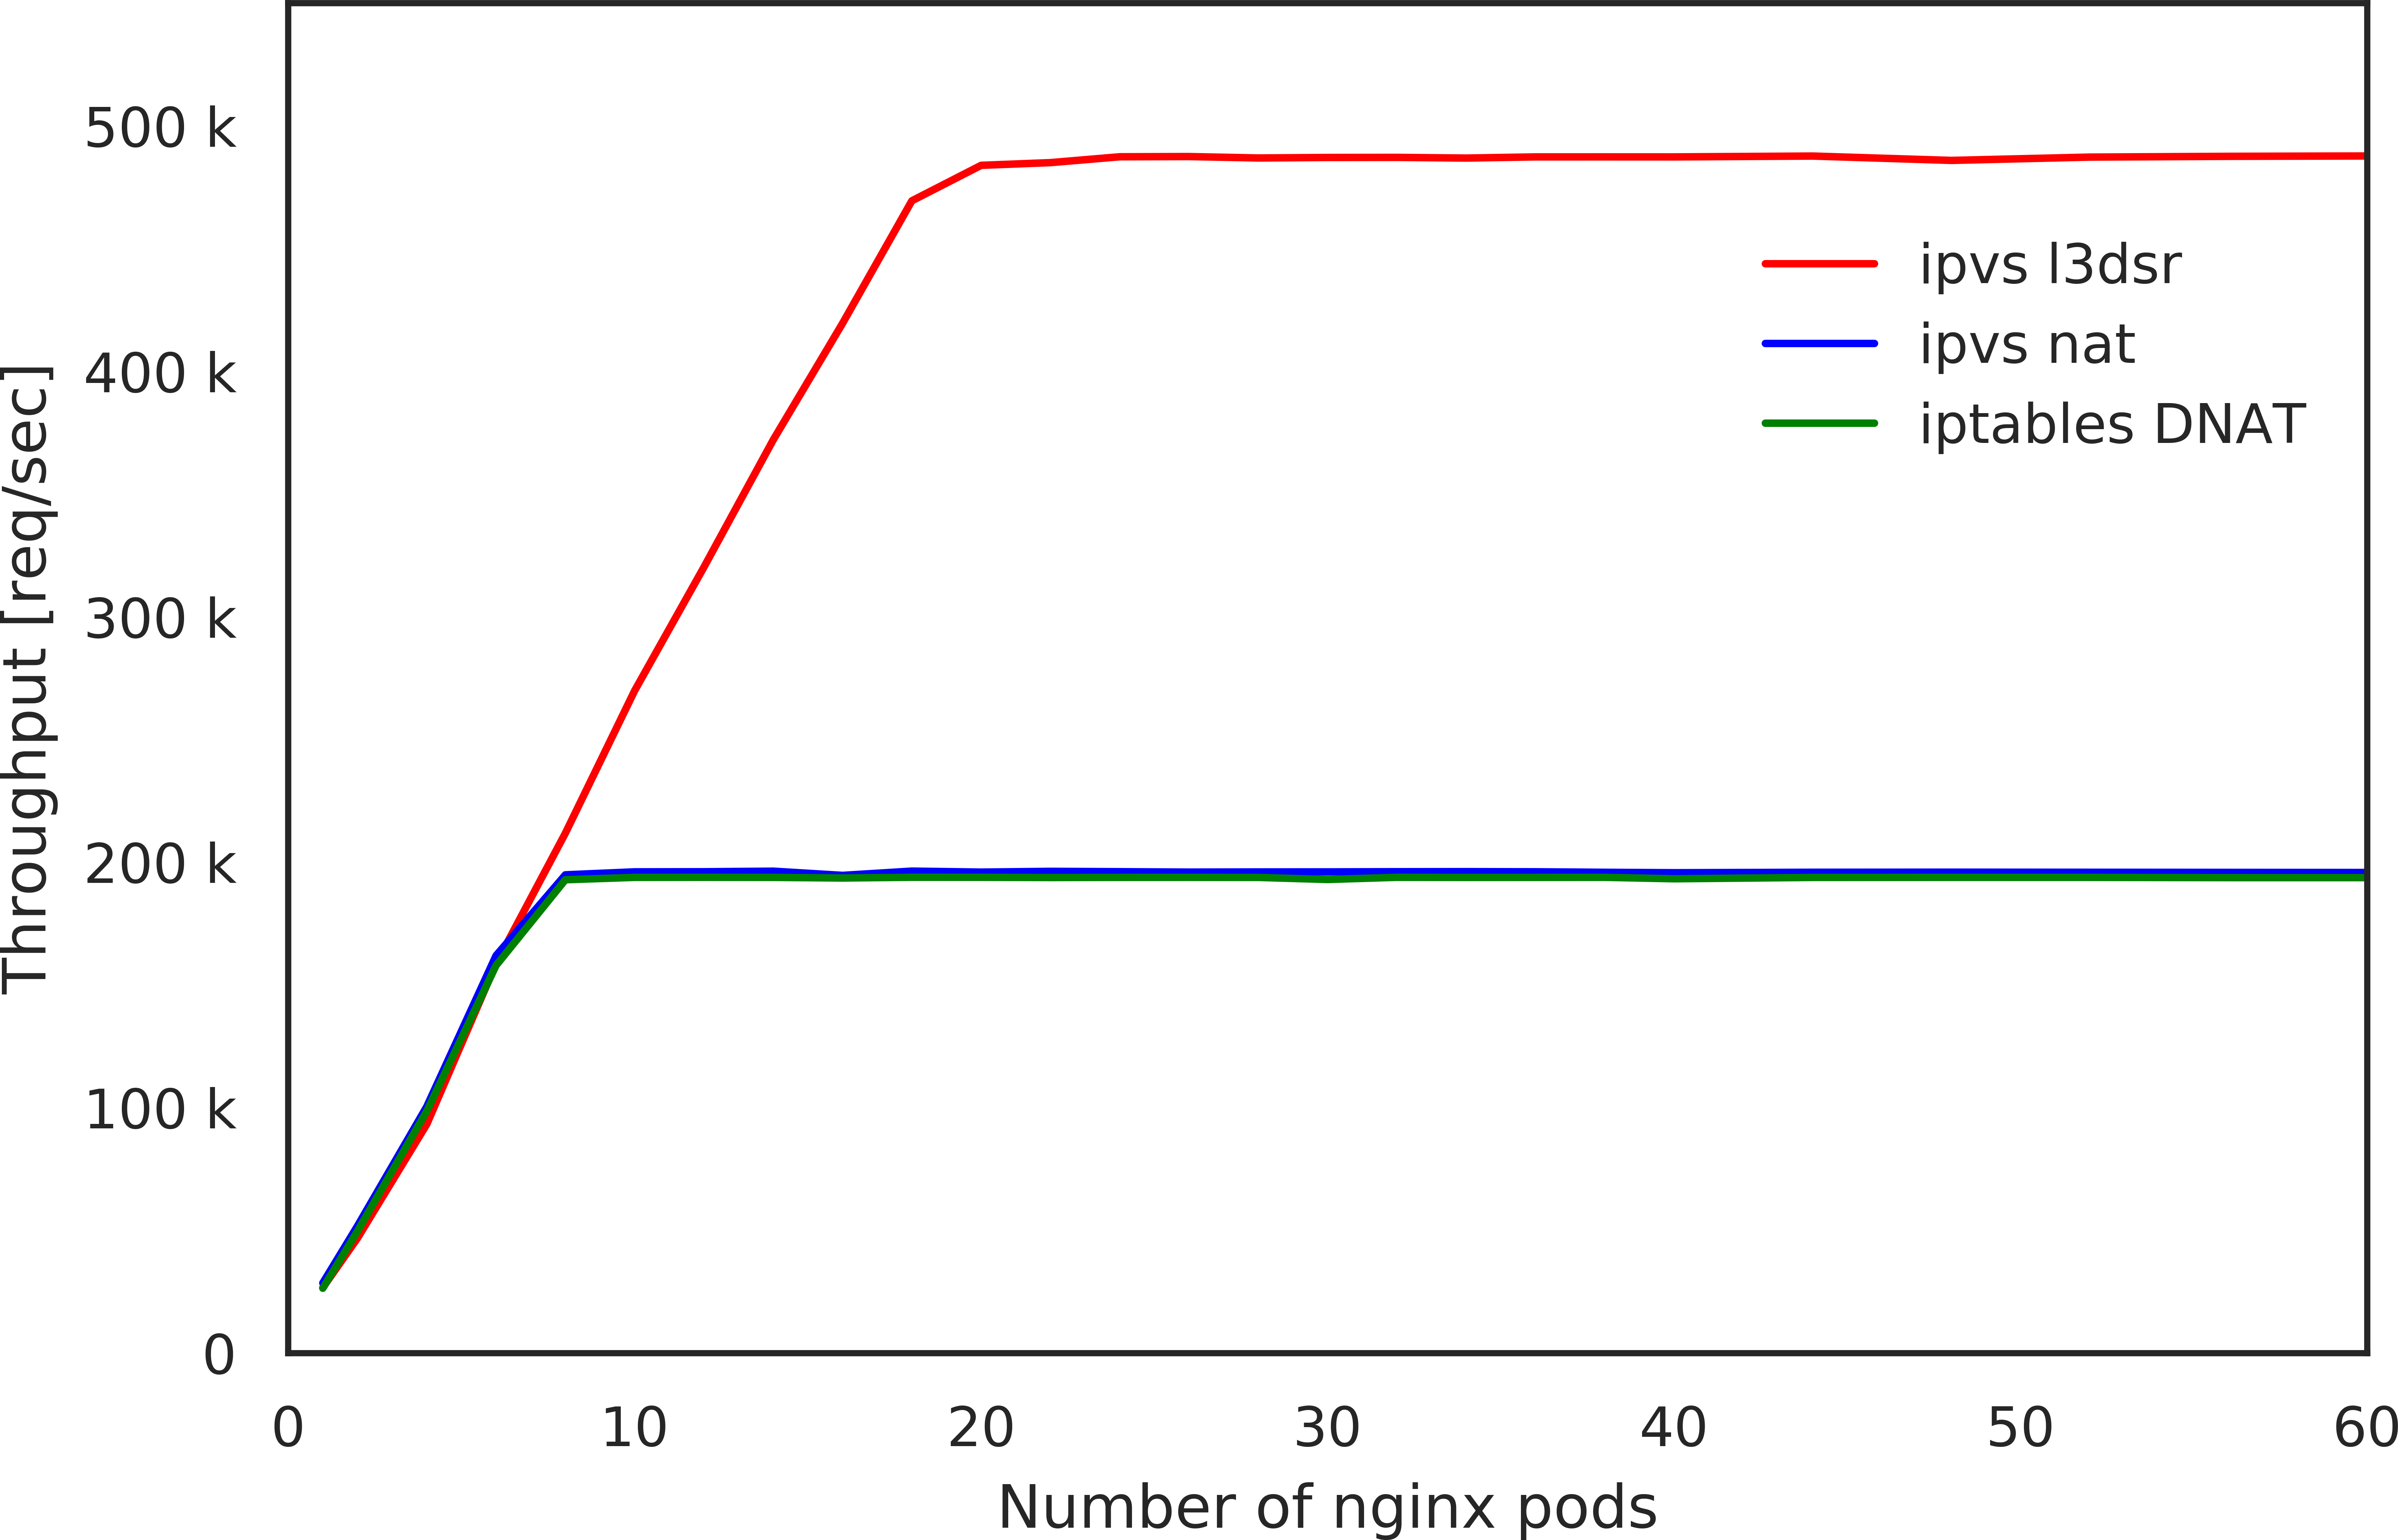
\includegraphics[width=0.8\columnwidth]{Figs/ipvs_l3dsr_1g.png}
  \caption{Throughput of ipvs l3dsr @1Gbps.}
  \label{fig:ipvs_l3dsr_1g.png}
\end{figure}

The author carried out throughput measurement using the physical setup shown in Figure~\ref{fig:bench_1g_l3dsr}.
Figure~\ref{fig:ipvs_l3dsr_1g.png} shows the throughput of the ipvs-tun, conventional ipvs (after here the author call it ipvs-nat) and iptables DNAT.
As can be seen in the figure, while the performance levels for ipvs-nat and iptables DNAT exactly match, the performance levels for ipvs-tun is greatly improved, e.g., 1.5 times larger saturated throughput than for ipvs-nat and iptables DNAT cases.

\FloatBarrier

%\section{IEICE}

\subsection{Cloud Experiment}

\begin{figure}[h]

  \begin{subfigure}[t]{\columnwidth}
    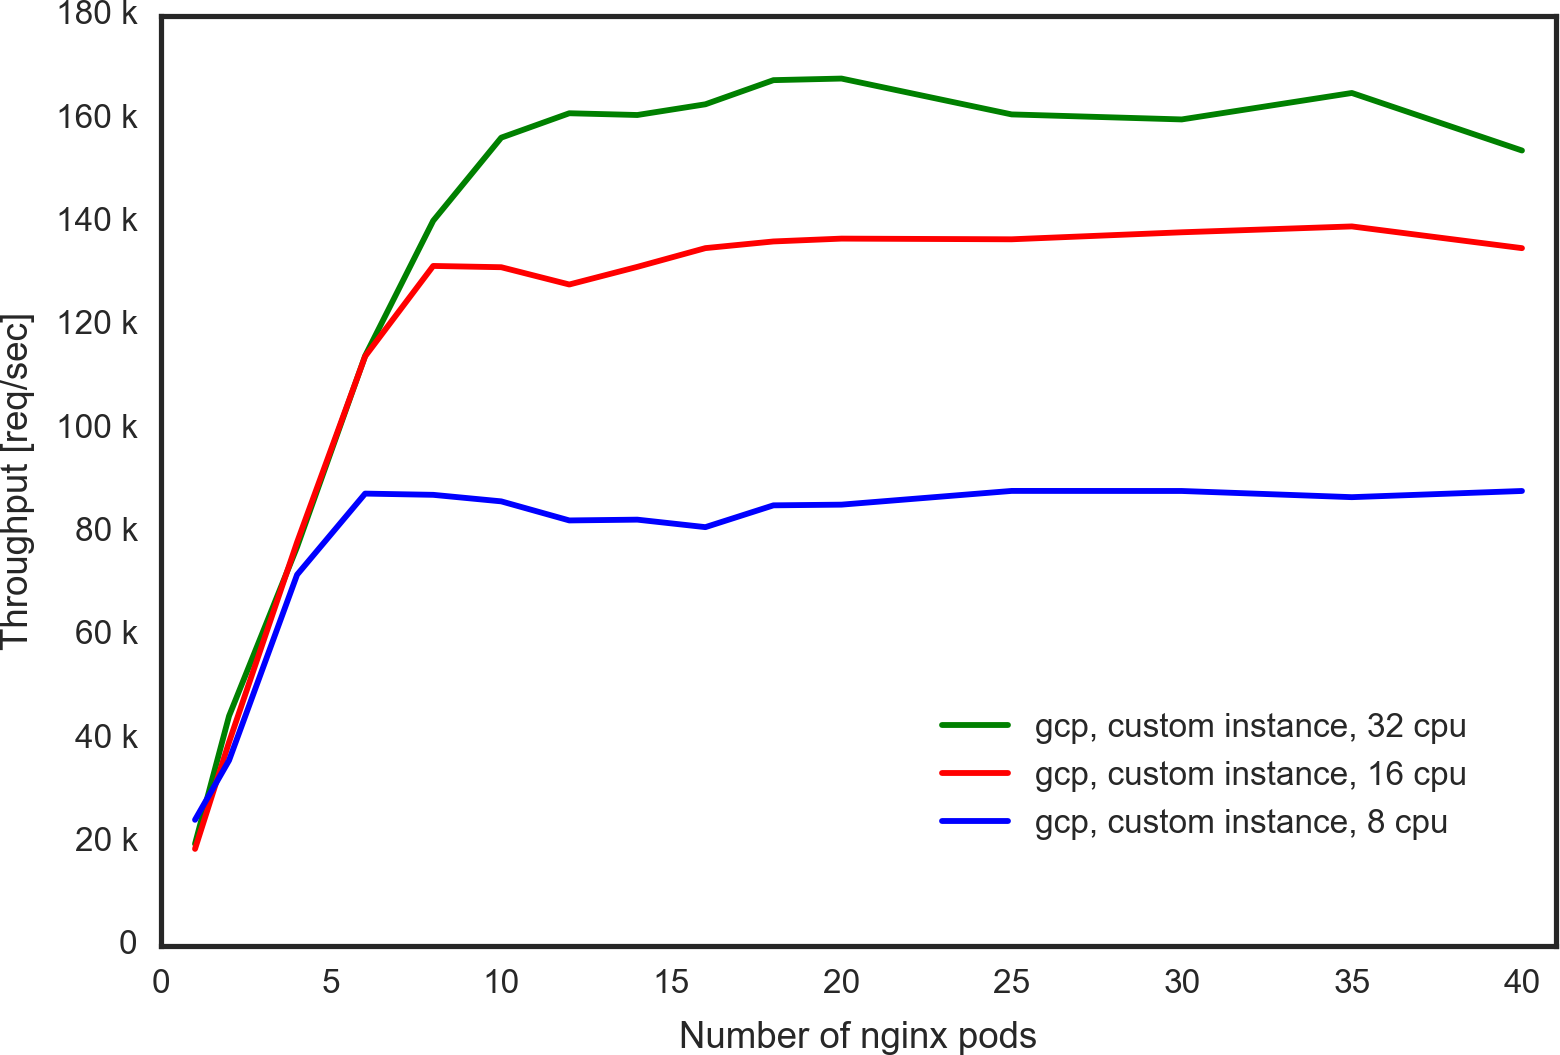
\includegraphics[width=0.9\columnwidth]{Figs/gcp_all_ieice}
    \caption{Througput in GCP}
    \label{fig:gcp_all_ieice}
  \end{subfigure}

  \par\bigskip

  \begin{subfigure}[t]{\columnwidth}
    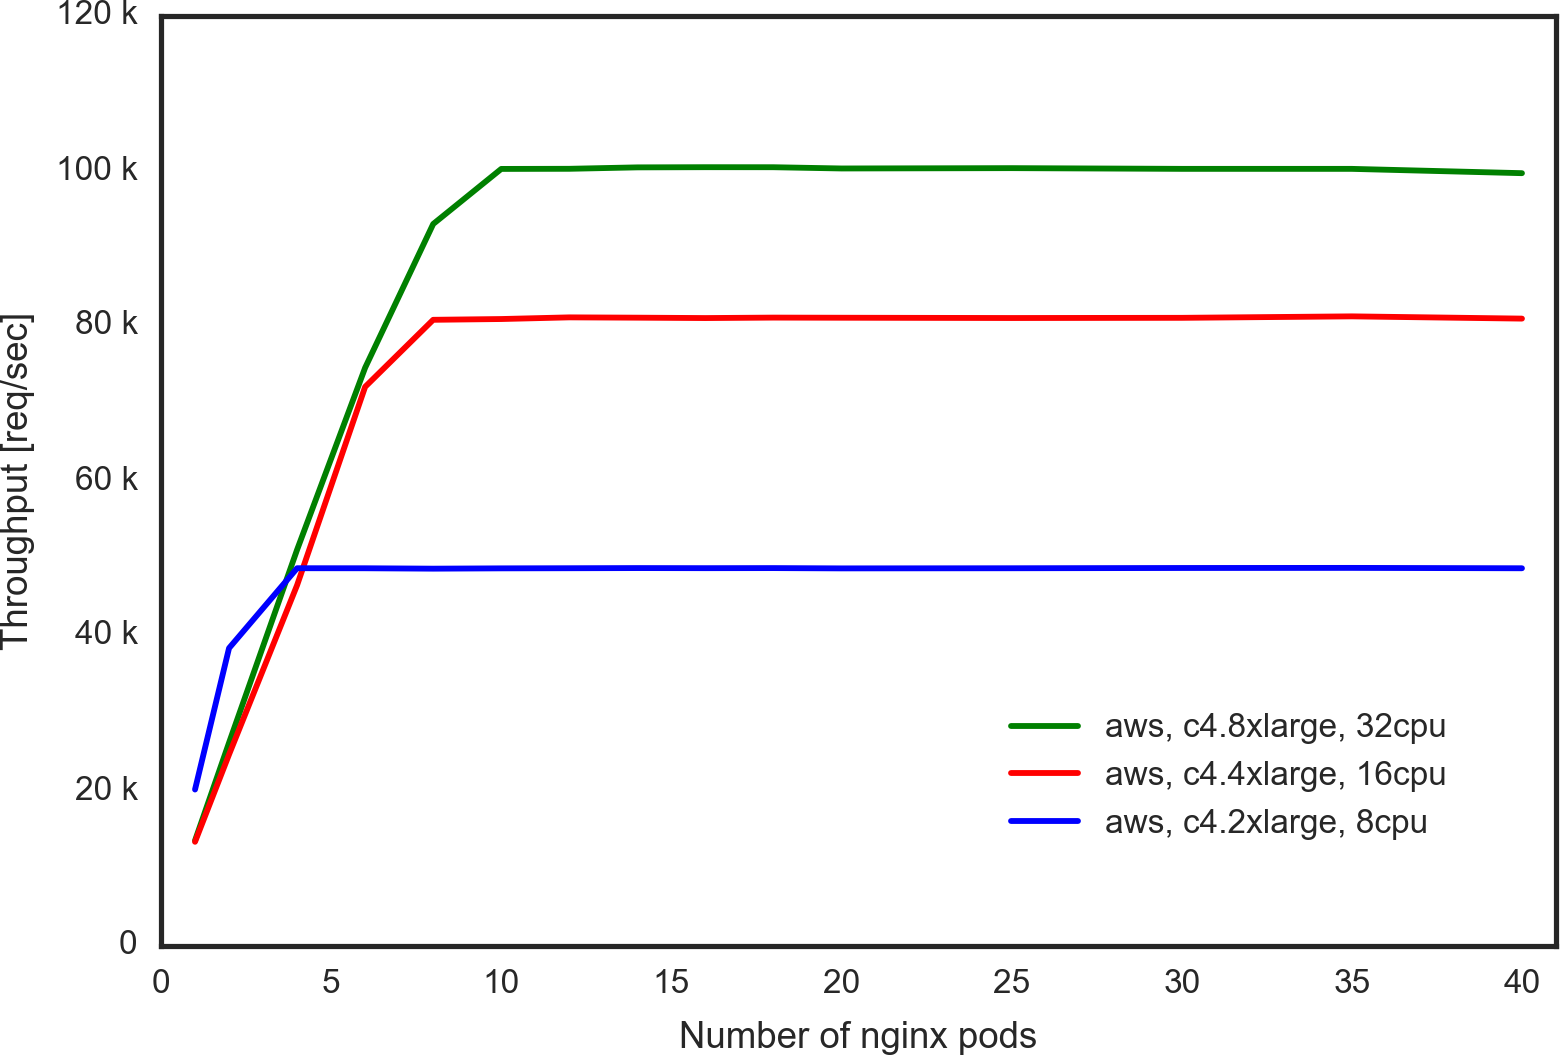
\includegraphics[width=0.9\columnwidth]{Figs/aws_c4_ieice}
    \caption{Througput in AWS}
    \label{fig:aws_c4_ieice}
  \end{subfigure}

  \caption[Throughput measurement results in cloud infrastructures]{Throughput measurement results in cloud infrastructures.}
  \label{fig:cloud_ipvs_performance}

\end{figure}

Fig.~\ref{fig:ipvs_performance}~(\subref{fig:gcp_all_ieice}) and Fig.~\ref{fig:ipvs_performance}~(\subref{fig:aws_c4_ieice}) show the load balancer performance levels that are measured in GCP and AWS, respectively. In the case of GCP, custom instance with 32Gbyte memory and with 8, 16, and 32 CPU are used.
And in the case of AWS instance type of c4.2xlarge, c4.4xlarge, and c4.8xlarge are used.
These are aimed to show that our proposed load balancer can be run in cloud environments and also functions properly.

Both results show similar characteristics as the experiment in an on-premise data center in Fig.~\ref{fig:ipvs_performance}~(\subref{fig:ipvs-iptables-nginx}), where throughput increased linearly to a certain saturation level that is determined by either network speed or machine specifications.
Since in the cases of cloud environments we can easily change the machine specifications, especially CPU counts, we measured throughput with several conditions of them.
From the first look of the results, since changing CPU counts changed the load balancer's throughput saturation levels, we thought VM's computation power limited the performance levels.
However, since there are cases in the cloud environment, where changing the VM types or CPU counts also changes the network bandwidth limit, a detailed analysis is further required in the future to clarify which factor limits the throughput in the cases of these cloud environments.
Still, we can say that the proposed ipvs load balancers can be run in GCP and AWS, and function properly.

\FloatBarrier

\section{Redundancy with ECMP}

The ECMP technique is expected to make the load balancers redundant and scalable since all the load balancer containers act as active.
We examined the behavior of the ECMP routing table updates, by changing the number of the load balancers.
After that, in order to explore the scalability, we also measured the throughput from a benchmark client with ECMP routes when multiple of the ipvs container load balancers are deployed.

\begin{figure}[h]
  \centering
  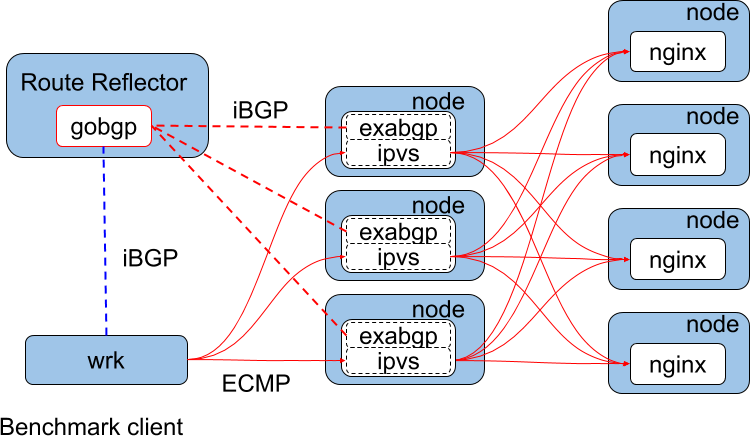
\includegraphics[width=0.9\columnwidth]{Figs/lb_ecmp_schem}

  \centering
  \begin{minipage}{0.9\columnwidth}
    \caption[Benchmark setup]{Benchmark setup.}
    \label{fig:ecmp-benchmark-schem}
  \end{minipage}
\end{figure}

{
\setlength{\tabcolsep}{1em}
\renewcommand{\arraystretch}{1.2}

\begin{table}[h]
  \centering
  \begin{tabular}{ll}
    \hline 
    \multicolumn{2}{l}{[Hardware Specification]}   \\
    & CPU: Xeon E5-2450 2.10GHz x 8 (with Hyper Threading) \\
    & Memory: 32GB \\
    & NIC: Broadcom BCM5720 Giga bit \\
    & (Node x 6, Load Balancer x 4) \\
    & \\
    & CPU: Xeon E5-2450 2.10GHz x 8 (with Hyper Threading) \\
    & Memory: 32GB \\
    & NIC: Intel X550 \\
    & (Client x 1) \\
    & \\
    \multicolumn{2}{l}{[Node Software]}  \\
    & OS: Debian 9.5, linux-4.16.8 \\
    & Kubernetes v1.5.2 \\
    & flannel v0.7.0 \\
    & etcd version: 3.0.15 \\
    & \\
    \multicolumn{2}{l}{[Container Software]}   \\
    & Keepalived: v1.3.2 (12/03,2016) \\
    & nginx : 1.15.4(web server) \\
  \hline 
  \end{tabular}
  \caption{Hardware and software specifications.}
  \label{tab:ecmp-hw_sw_spec}
\end{table}
}

Fig.~\ref{fig:ecmp-benchmark-schem} shows the schematic diagram of the experimental setup and also summarizes hardware and software specifications.
Notable differences from the previous throughput experiment in Fig.~\ref{fig:benchmark-schem} are as follows;
1) Each load balancer pods now consists of both an ipvs container and an exabgp container.
2) The routing table of the benchmark client is updated by BGP protocol through a route reflector.
3) The NIC of the benchmark client has been changed to 10 Gbps card since now we have multiple of ipvs container load balancers that are capable of filling up 1 Gbps bandwidth.
4) Some of the software have been updated to the most recent versions at the time of the experiment.

\FloatBarrier

{
\setlength{\tabcolsep}{1em}
\renewcommand{\arraystretch}{1.2}

\begin{table}[h]

  \begin{subtable}{.9\textwidth}
    \centering
    \begin{tabular}{l}
    \hline 
    10.1.1.0/24 via 10.0.0.106 dev eth0 proto zebra metric 20 \\
    \hline
    \end{tabular}
    \caption{With single load balancer {\em pod}.}
    \label{tab:single}
  \end{subtable}

  \par\bigskip

\begin{subtable}{.9\textwidth}
  \centering
  \begin{tabular}{ll}
    \hline
    \multicolumn{2}{l}{10.1.1.0/24 proto zebra metric 20 } \\
    \hspace{15 mm}
    & nexthop via 10.0.0.105  dev eth0 weight 1 \\
    & nexthop via 10.0.0.106  dev eth0 weight 1 \\
    & nexthop via 10.0.0.107  dev eth0 weight 1 \\
    \hline
  \end{tabular}
  \caption{With three load balancer {\em pod}s.}
  \label{tab:three}
\end{subtable}

  \par\bigskip

\begin{subtable}{.9\textwidth}
  \centering
  \begin{tabular}{ll}
    \hline
    \multicolumn{2}{l}{10.1.1.0/24 pro to zebra metric 20 } \\
    \hspace{15 mm}
    & nexthop via 10.0.0.107  dev eth0 weight 1 \\
    & nexthop via 10.0.0.105  dev eth0 weight 1 \\
    & nexthop via 10.0.0.106  dev eth0 weight 1 \\
    \multicolumn{2}{l}{10.1.2.0/24 proto zebra metric 20 } \\
    \hspace{15 mm}
    & nexthop via 10.0.0.107  dev eth0 weight 1 \\
    & nexthop via 10.0.0.106  dev eth0 weight 1 \\
    \hline
  \end{tabular}
  \caption{For a service with three load balancer {\em pod}s and a service with two load balancer {\em pod}s.}
  \label{tab:double_svc}
\end{subtable}

\caption{ECMP routing tables.}
\label{tab:exabgp_routing_table}
\end{table}
}

First, we examined ECMP functionality by watching the routing table on the benchmark client.
Fig.~\ref{fig:exabgp_routing_table}~(\subref{fig:single}) shows the routing table entry on the router when a single load balancer pod exists.
From this entry, we can tell that packets toward 10.1.1.0/24 are forwarded to 10.0.0.106 where the load balancer pod is running.
It also shows that this routing rule is updated by zebra.

When the number of the load balancer pods is increased to three, we can see the routing table entry in Fig.~\ref{fig:exabgp_routing_table}~(\subref{fig:three}).
We have three next hops towards 10.1.1.0/24 each of which being the node where the load balancer pods are running.
The weights of the three next-hops are all 1.
The update of the routing entry was almost instant as we increased the number of the load balancers.

Fig.~\ref{fig:exabgp_routing_table}~(\subref{fig:double_svc}) shows the case where we additionally started new service with two load balancer pods with service addresses in 10.1.2.0/24 range.
We could accommodate two different services with different service IPs, one with three load balancers and the other with two load balancers on a group of nodes(10.0.0,105,10.0.0,106,10.0.0,107).
The update of the routing entry was almost instant as we started the load balancers for the second service.

As far as the route withdrawal is concerned, if an exabgp is killed by SIGKILL or SIGTERM the kernel of the node close the BGP connection by sending out a packet with FIN flag to the peer gobgpd on the route reflector, and thus the route is withdrawn immediately.
The gobgp on the route reflector also periodically check the BGP connection, and if the peer exabgp container is unresponsive for more than the specified duration, “hold-time“ setting in gobgpd, it will also terminate the connection and withdraw the route.
The packets arriving within the duration will be dropped.
However, we can set up the “hold-time” short enough so that the retransmitted TCP packets from the client will be forwarded correctly to functioning load balancers.

\FloatBarrier

\begin{figure}[h]
  \centering
  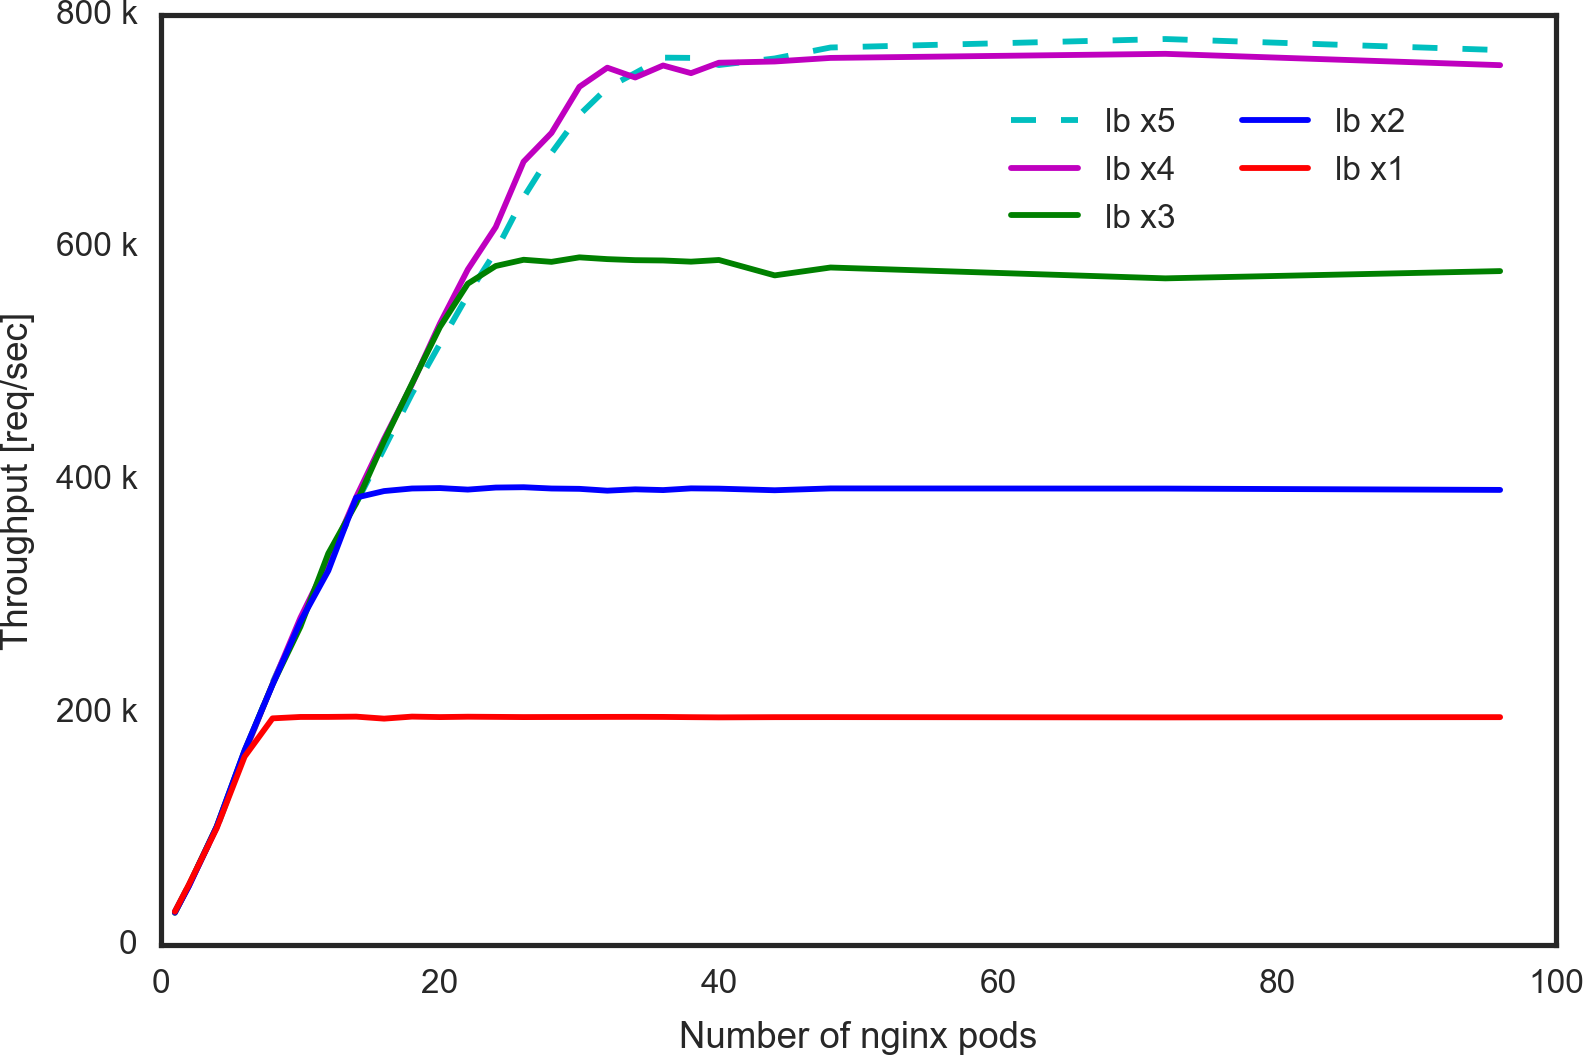
\includegraphics[width=0.9\columnwidth,left]{Figs/ecmp_lb_cubic_ieice}
  \centering
  \begin{minipage}{0.9\columnwidth}
        \caption[Throughput of ECMP redundant load balancer]{
          Throughput of ECMP redundant load balancer.
          The throughputs are measured for a single load balancer(lb x1), two(lb x2), three(lb x3) and four(lb x4) load balancers.
        }
  \end{minipage}
  \label{fig:ecmp_lb_cubic_ieice}
\end{figure}

\begin{figure}[h]
  \centering
  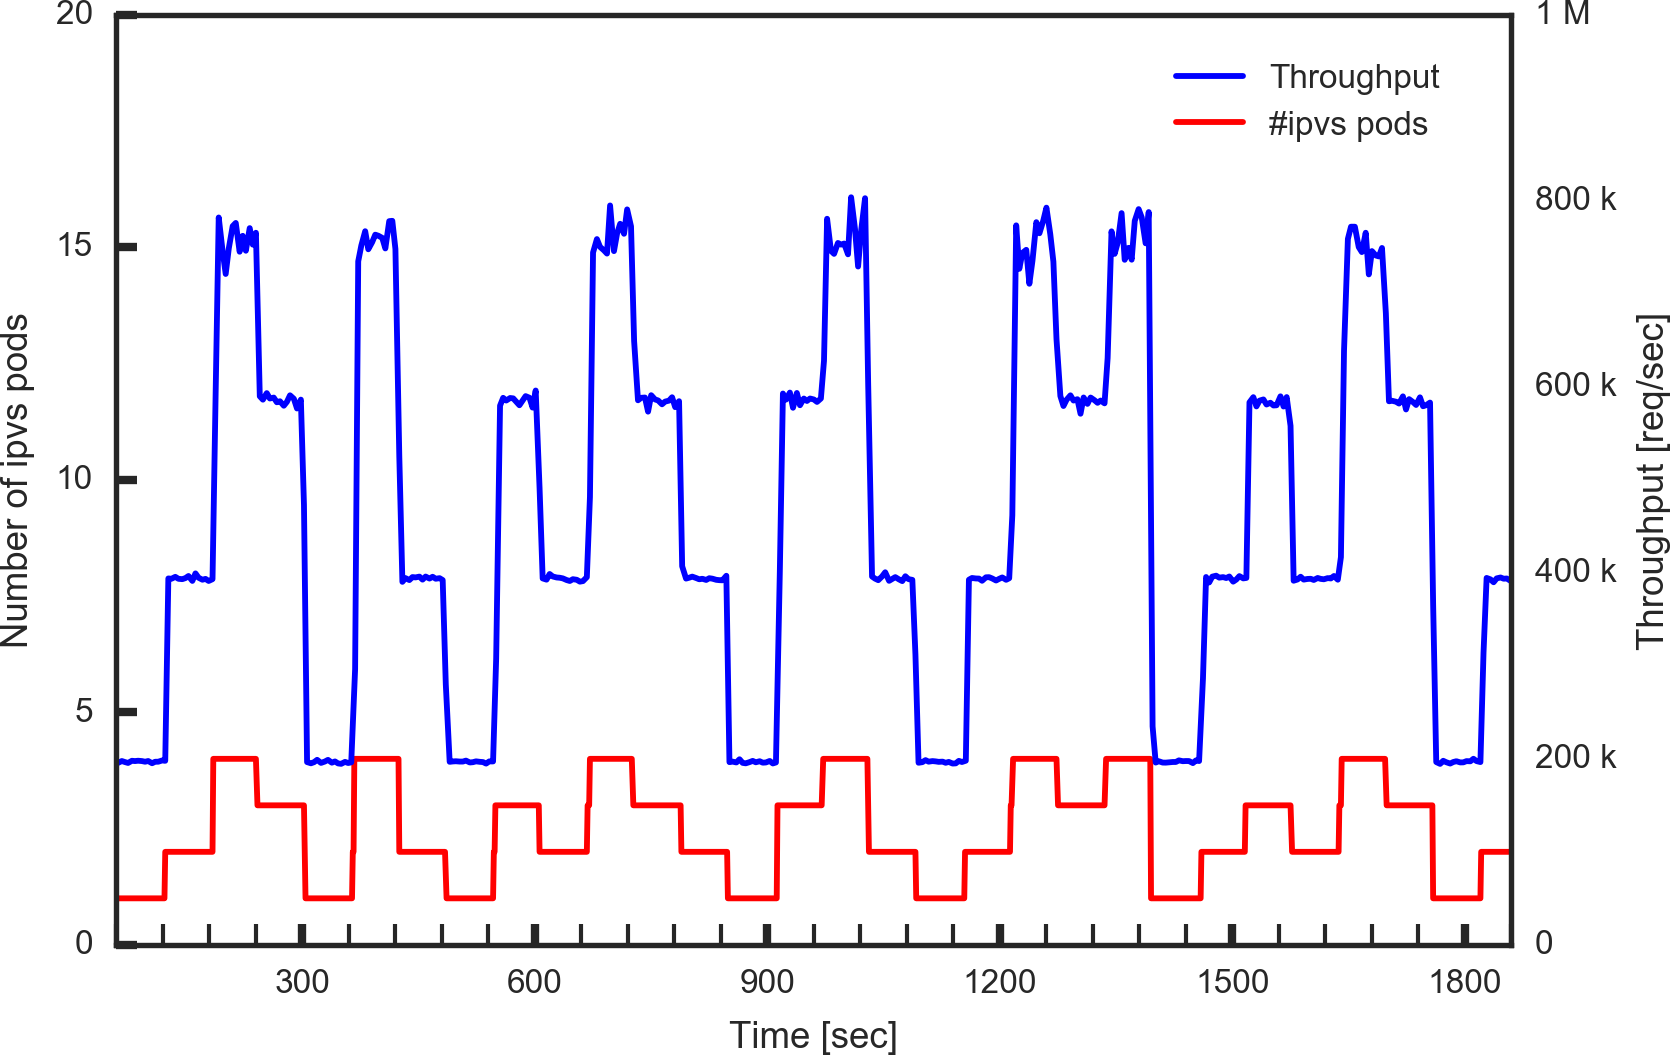
\includegraphics[width=0.98\columnwidth,left]{Figs/ecmp_response_ieice}
  \centering
  \begin{minipage}{0.9\columnwidth}
    \caption[Throughput responsiveness]{
      Throughput responsiveness.
      This shows the throughput responsiveness when the number of the load balancers was changed randomly in every 60 seconds.
    }
  \end{minipage}
  \label{fig:ecmp_response_ieice}
\end{figure}


\begin{figure}[h]
  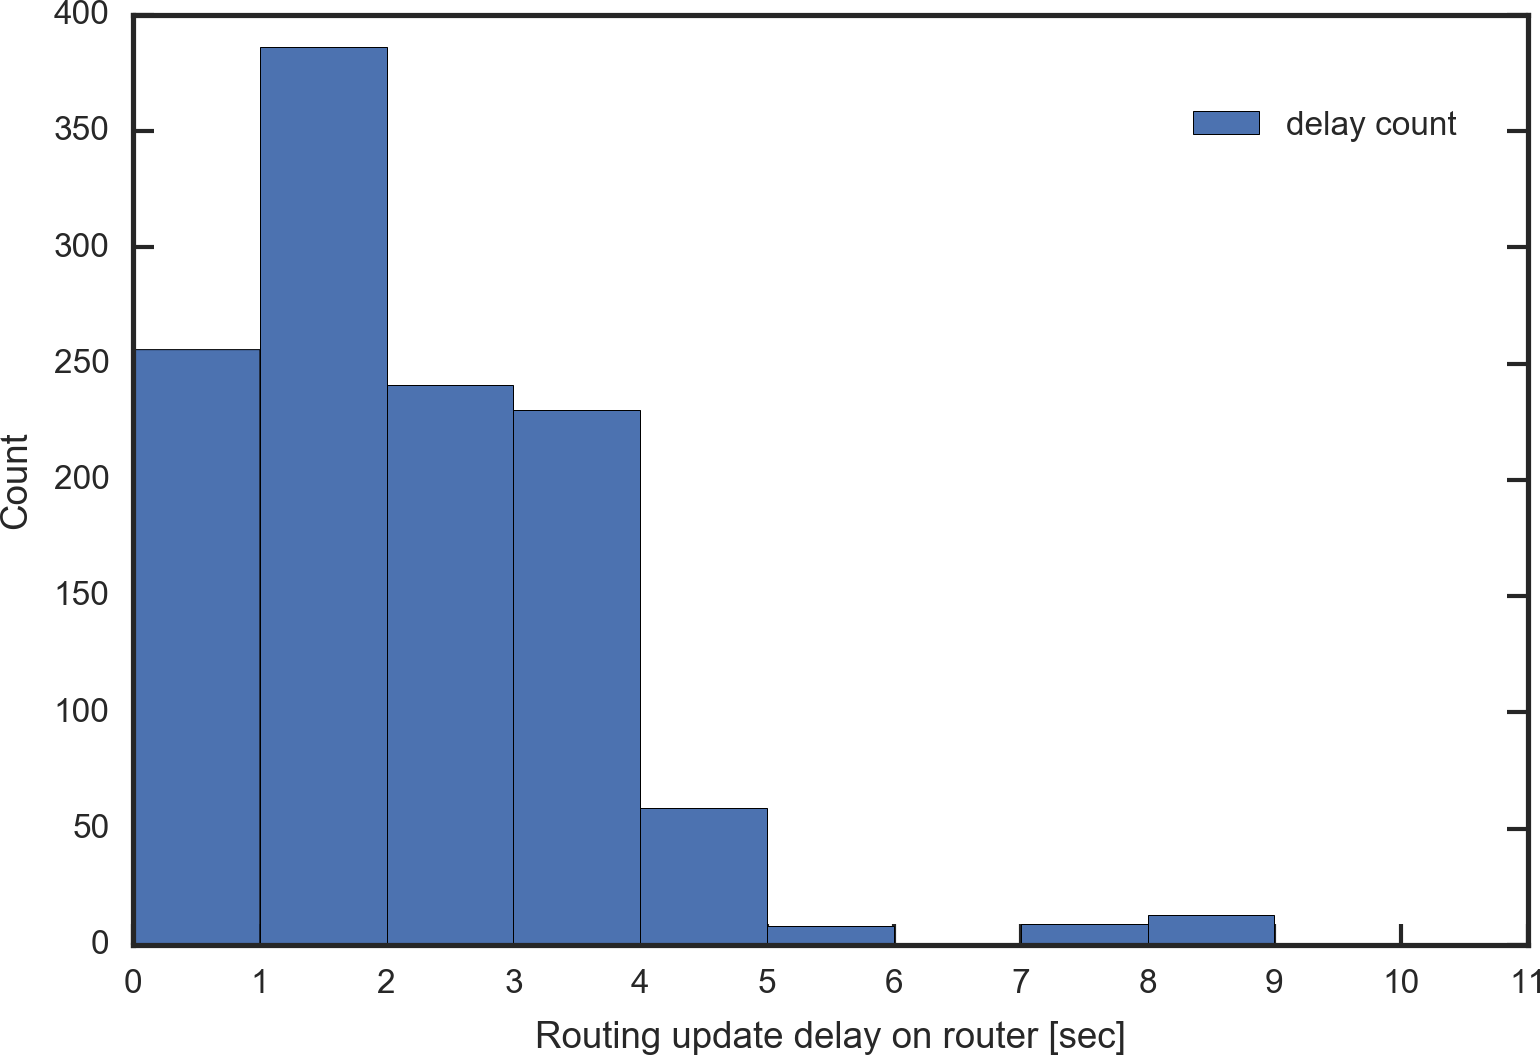
\includegraphics[width=0.9\columnwidth,left]{Figs/ecmp_delay_histgram_ieice}
  \centering
  \begin{minipage}{0.9\columnwidth}
    \caption[A histogram of the ECMP update delay]{
      A histogram of the ECMP update delay.
      This shows the delays until the number of running ipvs pods is reflected into the routing table on the benchmark client,
    when the number of the ipvs pods is changed randomly every 60 seconds for 20 hours.
    }
  \end{minipage}
  \label{fig:ecmp_delay_histgram_ieice}
\end{figure}

We also carried out throughput measurement to show that our proposed architecture increases the throughput as we increase the number of the load balancers.
Fig.~\ref{fig:ecmp_scalability}~(\subref{fig:ecmp_lb_cubic_ieice}) shows the results of the measurements.
There are four solid lines in the figure, each corresponding the throughput result when there are one through four of the proposed load balancers.
The saturated levels, i.e. performance levels depend on the number of the ipvs load balancer pods(lb x 1 being the case with one ipvs pods, and lb x2 being two of them and as such). The performance level increases linearly as we increases the number of the load balancers up to four of the ipvs load balancers, but did not scale further.
This was because we used up CPU power of the benchmark client since the CPU usage was 100\% when there were more than four load balancers.
We expect that replacing the benchmark client with more powerful machines, or changing the experimental setup so that multiple benchmark clients can access the load balancers through an ECMP router, will improve the performance level further.

Fig.~\ref{fig:ecmp_scalability}~(\subref{fig:ecmp_response_ieice}) shows the throughput measurement results when we periodically changed the number of the load balancers. 
The red line in the figure shows the number of the ipvs load balancer pods, which we changed randomly every 60 seconds.
The blue line corresponds to the resulting throughput.
As we can see from the figure, the blue line nicely follows the shape of the red line.
This indicates that new load balancers are immediately utilized after they are created, and after removing some load balancers, the traffic to them is immediately directed to the existing load balancers.

Fig.~\ref{fig:ecmp_scalability}~(\subref{fig:ecmp_delay_histgram_ieice}) shows histogram of the ECMP update delay, where we measured the delays until the number of running ipvs pods is reflected in the routing table on the benchmark client, as we change the number of the ipvs pods randomly every 60 seconds for 20 hours.
As we can see from the figure, most of the delays are within 6 seconds, and the largest delay during the 20 hours experiment was 10 seconds.
We can conclude that ECMP routing update in our proposed architecture is quick enough.

\FloatBarrier

\section{Summary}\label{Conclusions}

In this paper, we proposed a portable load balancer with ECMP redundancy for the Kubernetes cluster systems that is aimed at facilitating migration of container clusters for web services.
We implemented an experimental web cluster system with multiple of load balancers and web servers using Kubernetes and OSSs on top of standard Linux boxes to prove the functionality of the proposed architecture.
We conducted performance measurements and found that the ipvs based load balancer in container functioned properly both in on-premise data center and cloud environments while it showed the comparable performance levels as the existing iptables DNAT based load balancer.
We also carried out experiments to verify the feasibility of ECMP redundancy in on-premise data center, and revealed that it functions properly with linear scalability up to four load balancers.

The current limitations of this study are;
1) Currently, BGP peering is not supported in GCP and AWS, and thus redundancy is achieved only by route update through cloud API upon the start of a load balancer.
The authors expect the cloud providers to support it in the future.
2) Most of the experiments are in 1Gbps network environments.
For future work, we plan to carry out throughput measurement in 10Gbps network environments and also improve the performance of a single software load balancer on standard Linux box using XDP technology.
